\chapter{\ifproject%
\ifenglish Project Structure and Methodology\else โครงสร้างและขั้นตอนการทำงาน\fi
\else%
\ifenglish Project Structure\else โครงสร้างของโครงงาน\fi
\fi
}

ในบทนี้จะกล่าวถึงหลักการ และการออกแบบระบบ

\makeatletter

% \renewcommand\section{\@startsection {section}{1}{\z@}%
%                                    {13.5ex \@plus -1ex \@minus -.2ex}%
%                                    {2.3ex \@plus.2ex}%
%                                    {\normalfont\large\bfseries}}

\makeatother
%\vspace{2ex}
% \titleformat{\section}{\normalfont\bfseries}{\thesection}{1em}{}
% \titlespacing*{\section}{0pt}{10ex}{0pt}

\section{โครงสร้างของเว็บไซต์}
โปรเจคนี้จะแบ่งออกเป็น 3 ส่วน
\begin{enumerate}
  \item Fontend - ใช้ React ในการจัดการหน้าเว็ปไซต์
  \item Backend - ใช้ Nest เป็นตัวกลางในการสื่อสารระหว่าง Fontend และ Database ด้วย API
  \item Database - ใช้การเก็บข้อมูลแบบ SQL โดยใช้ PostgreSQL และใช้ Firebase Cloud Storage ในการเก็บรูปภาพจากการอัพโหลด
\end{enumerate}

\begin{figure}[h]
  \begin{center}
  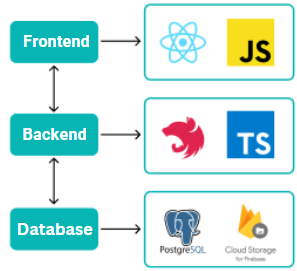
\includegraphics[width=6cm,height=6cm,keepaspectratio]{SWAReal.png}
  \end{center}
  \caption[โครงสร้างของเว็บไซต์]{โครงสร้างของเว็บไซต์}
  \label{fig:โครงสร้างของเว็บไซต์}
\end{figure}

\section{ฟีเจอร์}
\subsection{ฟีเจอร์การใช้งานของผู้เล่น}
การใช้งานในฝั่งผู้เล่นจะมีระบบหลักๆ ดังนี้
\begin{enumerate}
  \item ระบบสร้างทีม - ใช้สร้างทีมเพื่อเข้าร่วมการแข่งขันทัวร์นาเมนต์ต่างๆ โดยจะสร้างทีมเป็นของแต่ละเกมที่ต้องการแข่งแยกกัน เช่น ทีมValorant ก็จะใช้ลงทัวร์นาเมนต์ได้แค่เกม Valorant เท่านั้น
  \item ระบบจัดการทีม - ใช้จัดการคนในทีม รับคนเข้าทีม และแสดงประวัติการเล่นของทีม
  \item ระบบจัดการโปรไฟล์ - ใช้จัดการโปรไฟล์เปลี่ยนชื่อ แสดงข้อมูลการเข้าร่วมแข่งและทีม
  \item ระบบเลือก และสมัครทัวร์นาเมนต์ - เลือกทัวร์นาเมนต์ที่ต้องการแข่งขั้นสามารถดูรายละเอียด เลือกเกมที่ต้องการ และสมัครเข้าร่วมการแข่งขันได้
\end{enumerate}

\subsection{ฟีเจอร์การใช้งานของผู้จัดงาน}
การใช้งานในฝั่งผู้จัดการจะมีระบบหลักๆ ดังนี้
\begin{enumerate}
  \item ระบบสร้างจัดการทัวร์นาเมนต์ - ใช้สร้างทัวร์นาเมต์กำหนดรายระเอียดการแข่ง กฎกติกา เวลาแข่ง และรูปหน้าปกทัวร์นาเมนต์
  \item ระบบเดชบอร์ดในการจัดการทัวร์นาเมนต์ - ใช้ในการจัดการทัวร์นาเมนต์ผลแพ้ชนะ และคะแนน
  \item ระบบจัดตารางแข่ง - ใช้จัดการสายการแข่งโดยสามารถเลือกทีม และเวลาลงสายการแข่งได้ตามที่ต้องการ
\end{enumerate}

\section{ฐานข้อมูล}
ฐานข้อมูลที่ใช้ในโครงงานนี้จะมีด้วยกันทั้งหมด 9 tables ได้แก่
\begin{enumerate}
  \item User - ใช้ในการเก็บข้อมูลพื้นฐานของผู้ใช้
  \item Game - ใช้ในการเก็บข้อมูลเกมต่างๆเพื่อใช้เป็นข้อมูลในการสร้างทีม และทัวร์นาเมนต์
  \item Team - ใช้เก็บข้อมูล และรายเอียดของทีม
  \item Team Member - ใช้เก็บข้อมูลสมาชิกในทีมแต่ละทีม
  \item Team Request -  ใช้เก็บข้อมูลการขอเข้าสมัครเข้าร่วมทีมของแต่ละทีม
  \item Tournament - ใช้เก็บข้อมูล และรายละเอียดทัวร์นาเมนต์
  \item Tournament Join - ใช้เก็บข้อมูลทีมที่เข้าร่วมของแต่ละทัวร์นาเมนต์
  \item Match - ใช้เก็บข้อมูลเกมการแข่งขันว่าใครแข่งกับใครในแต่ละทัวร์นาเมนต์
  \item Match Results - ใช้เก็บข้อมูลผลการแข่งขันของแต่ละ Match
\end{enumerate}
\begin{figure}[h]
  \begin{center}
  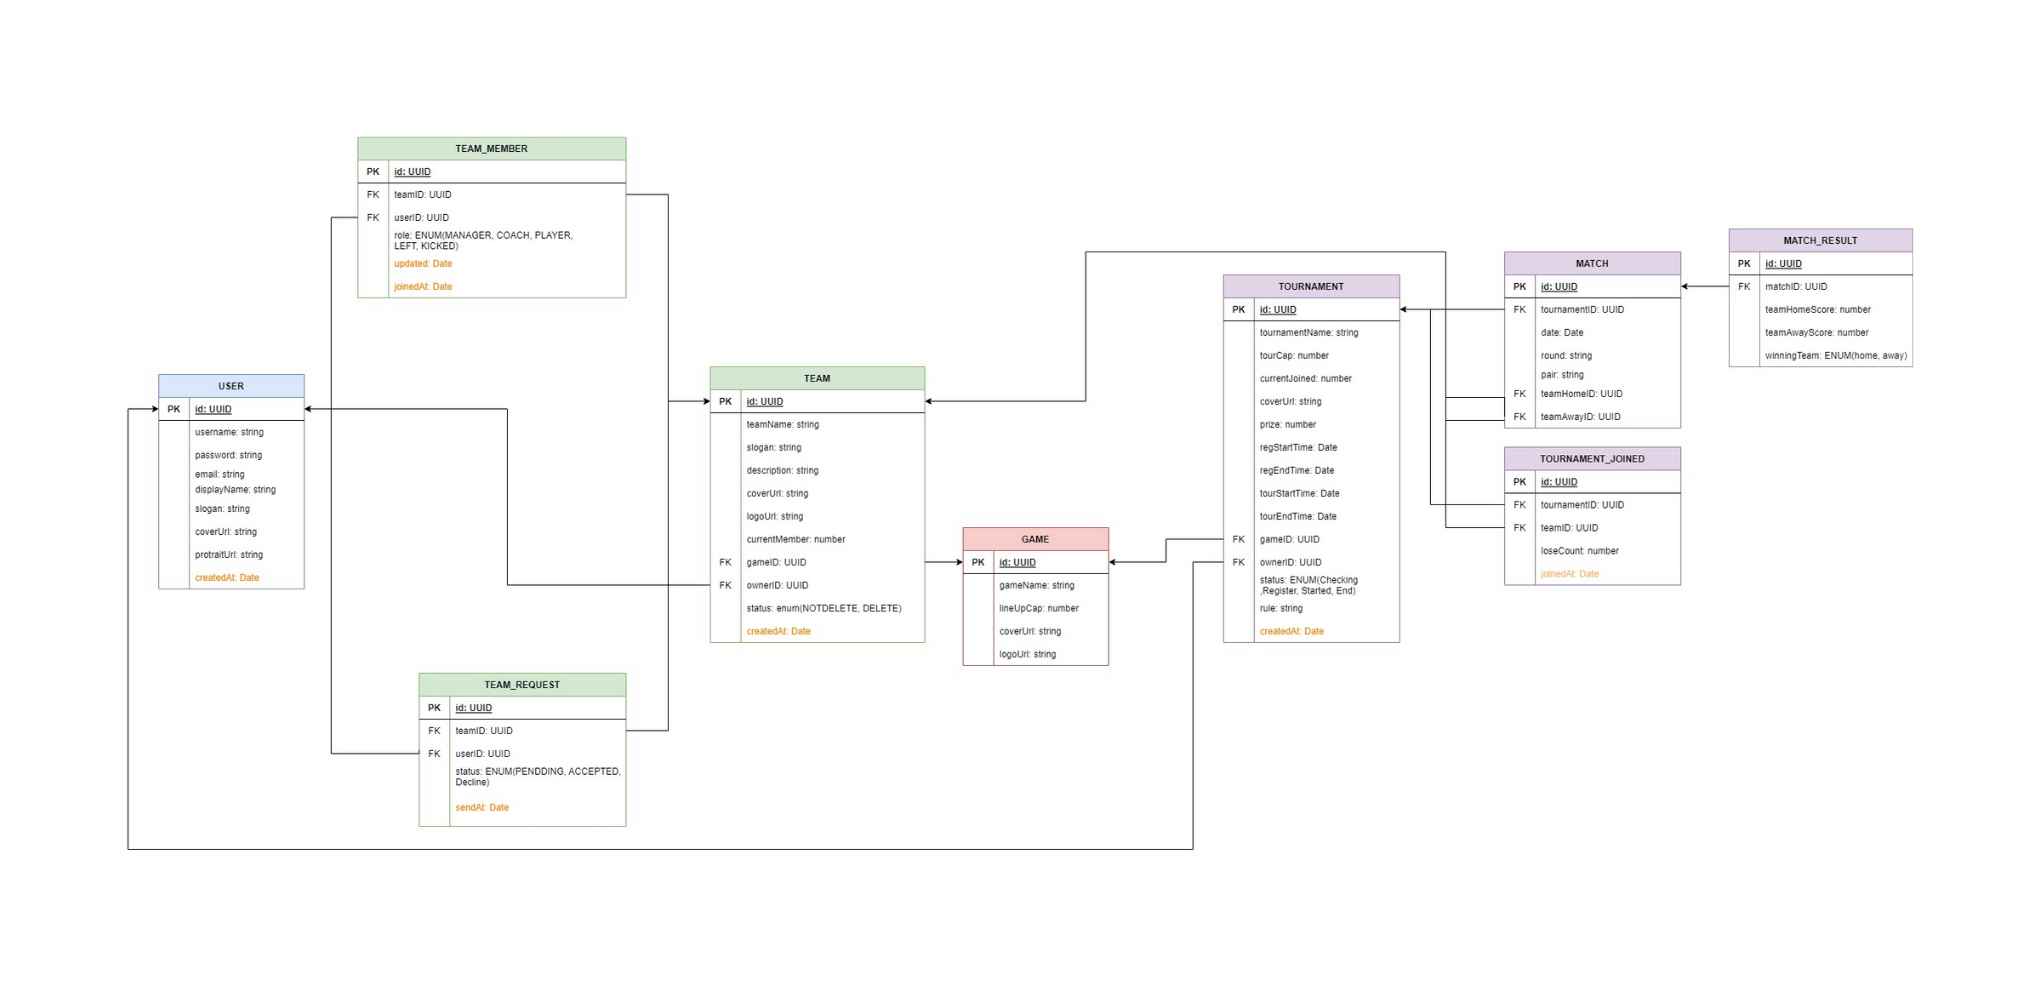
\includegraphics[width=18cm,height=6cm,keepaspectratio]{492_FyTy Tournament.png}
  \end{center}
  \caption[Database Schema]{Database Schema}
  \label{fig:Database Schema}
\end{figure}

\pagebreak

\section{authentication}
การที่จะเข้าถึง API Route ได้นั้นจะต้องมีการระบุตัวตนโดยใช้ JWT(JSON Web Token) โดยตัว JWT จะเข้ารหัสข้อมูลที่ส่งมาทำให้การส่งข้อมูลมีความปลอดภัย
โดยจะมีหลักการใช้งานดังนี้
\begin{enumerate}
  \item ผู้ใช้งานทำการ login เมื่อผู้ใช้งานทำการ login สำเร็จระบบจะนำ id ของ user ไปสร้าง token และส่งกลับไปยัง client
  \item ฝั่ง Client จะเซต Default การแนบ token มาด้วยทุกครั้งที่ทำการส่ง API Route มายัง server
  \item server จะตรวจเช็ค token ที่แนบมาก่อนว่า format ของ token เข้ารหัสถูกต้องหรือไม่ จาก secret key ที่เก็บไว้ในฝั่ง server หากถูกต้องจะทำการเข้าไปดูว่ามีข้อมูล user จริงหรือไม่จากค่า sub ที่แนบมากับ token
  \item เมื่อ token และ ข้อมูลถูกต้อง server จะคืนค่าข้อมูลจากฐานข้อมูลที่ต้องการให้
\end{enumerate}


\section{อินเตอร์เฟส และการทำงาน}
\subsection{หน้าโฮม}
เป็นหน้าแรกหลังจากเขามาในเว็ปไซต์โดยจะมี navbar ด้านบนใช้ในการนำทางไปในหน้าที่ต้องการ
แต่การที่จะไปหน้าอื่นได้นั้นต้องทำการ login ก่อนถึงจะสามารถไปได้โดยการ login นั้นสามารถใช้บัญชีที่สมัครกับทางเว็ปไซต์ได้ หรือจะใช้บัญชี Google ก็สามารถทำได้
\subsection{หน้าเดชบอร์ดทีม}
เป็นหน้าที่ใช้ในการค้นหาทีมโดยจะมีระบบในการค้นหาทีม และการกรองโดยสามารถกดเลือกจากการ์ดเกมต่างๆ หรือช่องค้นหาได้ และใช้ในการสร้างทีมโดยการสร้างทีมสามารถอัพโหลดรูปโลโก้ทีม และรูปปกทีมได้ตามความต้องการ
\subsection{หน้ารายละเอียดทีม}
เป็นหน้าที่จะบอกรายละเอียดของทีมนั้นว่าเคยไปแข่งทัวร์นาเมนต์อะไรไปแล้วบ้าง และมีสมาชิกในทีมเป็นใครบ้าง โดยแต่การ์ดที่แสดงรายละเอียดจะสามารถคลิกไปดูรายละเอียดได้โดยระบบจะทำการนำทางไปยังหน้าของรายละเอียดนั้นๆ
และถ้าหากเป็นเจ้าของทีมจะสามารถแก้ไขรูปทีม และรูปปกทีมได้
\subsection{หน้าแดชบอร์ดทัวร์นาเมนต์}
เป็นหน้าที่ใช้ในการค้นหาทีมโดยจะมีระบบในการค้นหาทัวร์นาเมนต์และการกรองโดยสามารถกดเลือกจากการ์ดเกมต่างๆ หรือช่องค้นหาได้ และใช้ในการสร้างทีมโดยการสร้างทีมสามารถอัพโหลดรูปโลโก้ทีม และรูปปกทีมได้ตามความต้องการ
\subsection{หน้ารายละเอียดทัวร์นาเมนต์}
เป็นหน้าที่จะแสดงรายละเอียดต่างๆของทัวร์นาเมนต์เช่น รายละเอียดเงินรางวัล เวลาแข่ง กฎกติกาการแข่ง ตารางเเข่ง และมีทีมอะไรบ้างที่เคยเข้าไปร่วมทีมด้วย
และถ้าหากเป็นเจ้าของทัวร์นาเมนต์เราจะสามารถแก้ไขภาพปกของทัวร์นาเมนต์ กฎกติกา จัดผู้เล่นลงสายได้ และสถานะของทัวร์นาเมนต์(register, start, end)
\subsection{หน้าสร้างทัวร์นาเมนต์}
เป็นหน้าที่แสดงทัวร์นาเมนต์ที่เราได้สร้างไปทั้งที่ยังดำเนินการอยู่ และที่จบไปแล้ว และเราสามารถสร้างทัวร์นาเมนต์ได้โดยกดไปที่ปุ่ม Create จากนั้นจะมี popup ขึ้นมาให้กรอกรายละเอียดเมื่อกรอกรายละเอียดเสร็จเรียบร้อยแล้วระบบจะนำทางไปยังหน้ารายละเอียดทัวร์นาเมนต์เพื่อใส่รายละเอียดเพิ่มเติมก่อนที่จะ public ทัวร์นาเมนต์นี้ให้ผู้อื่นสมัคร
\subsection{หน้าโปรไฟล์}
เป็นหน้าที่จะบอกรายละเอียดของผู้ใช้คนนั้นว่าเคยไปแข่งทัวร์นาเมนต์อะไรไปแล้วบ้าง และมีทีมอะไรบ้างที่เคยเข้าไปร่วมทีมด้วย โดยแต่การ์ดที่แสดงรายละเอียดจะสามารถคลิกไปดูรายละเอียดได้โดยระบบจะทำการนำทางไปยังหน้าของรายละเอียดนั้นๆ
และถ้าหากเป็นเจ้าของทีมจะสามารถแก้ไขรูปโปรไฟล์ และรูปปกได้
\subsection{หน้าตารางเวลาแข่ง}
เป็นหน้าที่จะแสดงเวลาการแข่งที่กำลังจะมาถึงโดยจะเรียงจากเวลาที่ใกล้ที่สุดก่อน และเมื่อเวลาผ่านไปจะถูกนำออกไม่นำมาแสดง


%  home
    \begin{figure}[ht]
      \begin{center}
      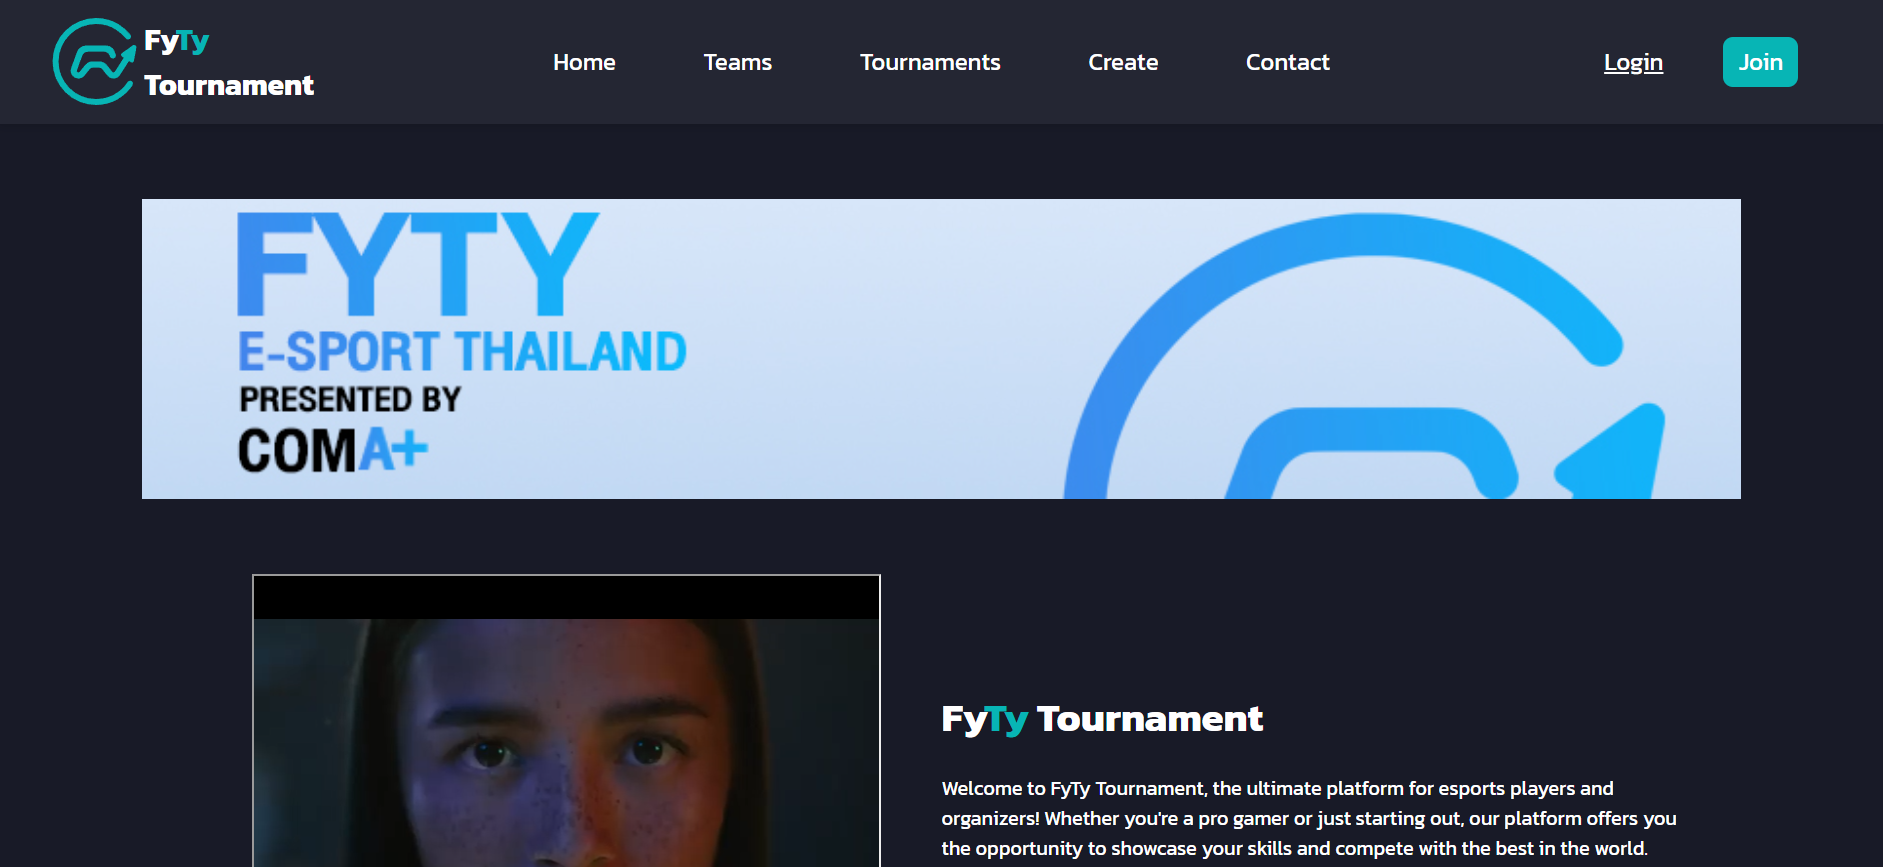
\includegraphics[width=18cm,height=7cm,keepaspectratio]{home_no_login.png}
      \end{center}
      \caption[หน้าโฮม]{หน้าโฮม}
      \label{fig:หน้าโฮม}
    \end{figure}
    \begin{figure}[ht]
      \begin{center}
        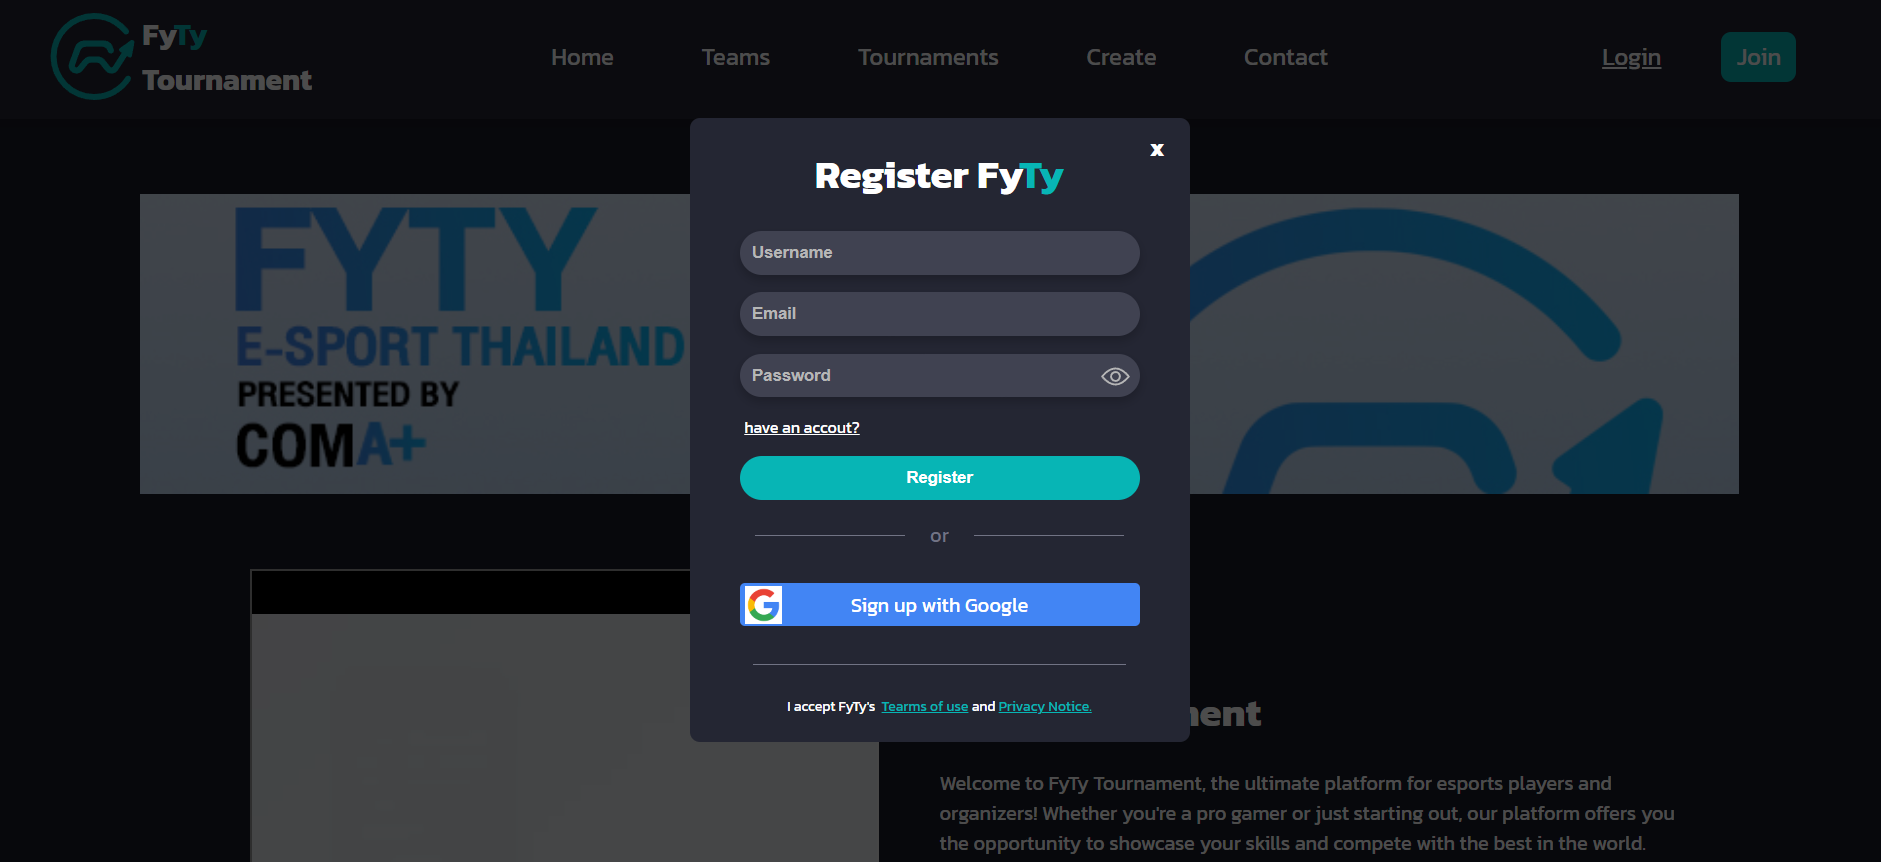
\includegraphics[width=18cm,height=7cm,keepaspectratio]{register.png}
      \end{center}
      \caption[Register Popup]{Register Popup}
      \label{fig:Register Popup}
    \end{figure}
    \begin{figure}[ht]
      \begin{center}
        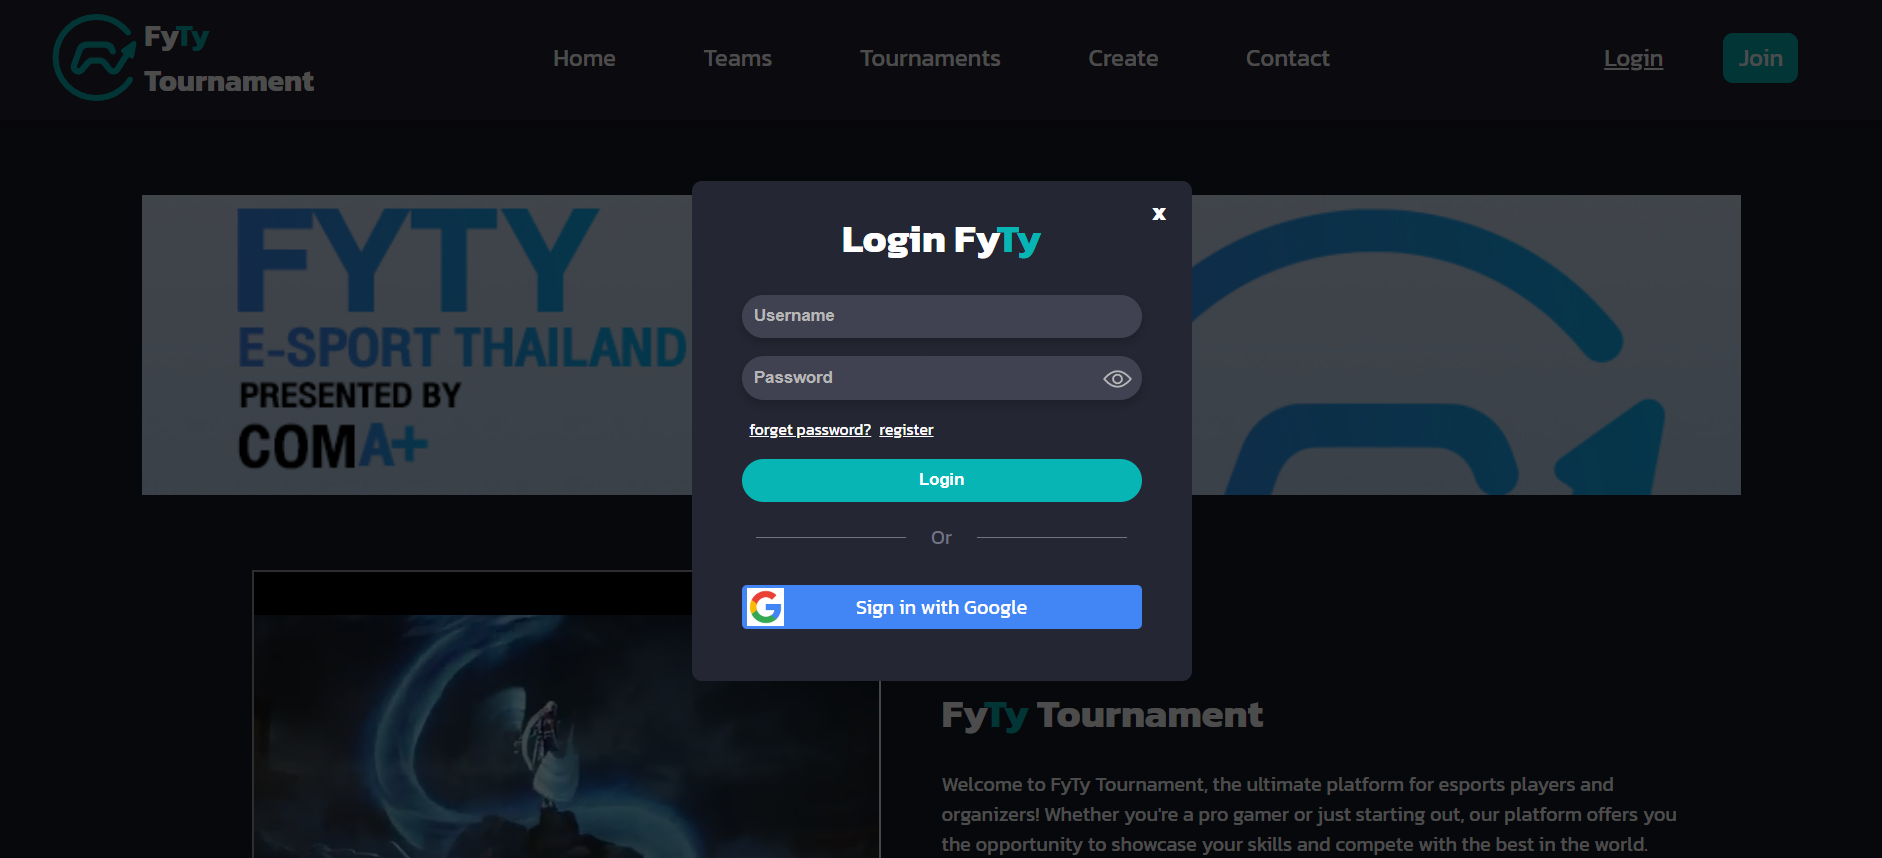
\includegraphics[width=18cm,height=7cm,keepaspectratio]{login.png}
      \end{center}
      \caption[Login Popup]{Login Popup}
      \label{fig:Login Popup}
    \end{figure}
    \begin{figure}[ht]
      \begin{center}
      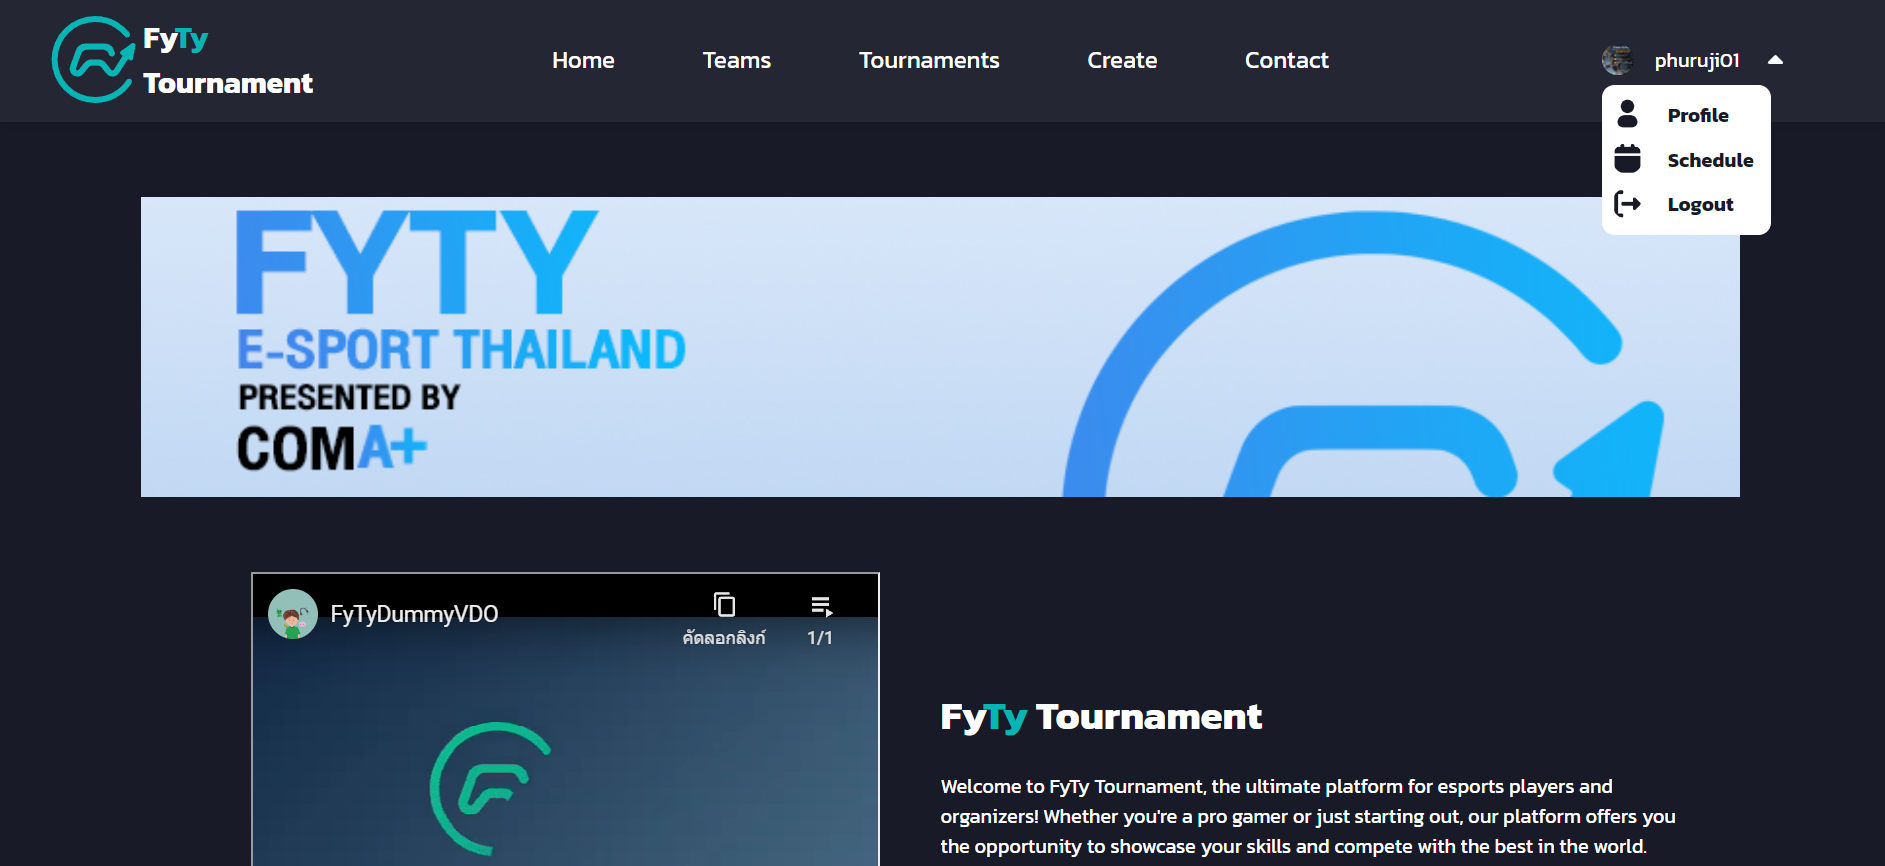
\includegraphics[width=18cm,height=7cm,keepaspectratio]{home_full.png}
      \end{center}
      \caption[หน้าโฮมหลังจาก Login]{หน้าโฮมหลังจาก Login}
      \label{fig:หน้าโฮมหลังจาก Login}
    \end{figure}
    \begin{figure}[ht]
      \begin{center}
      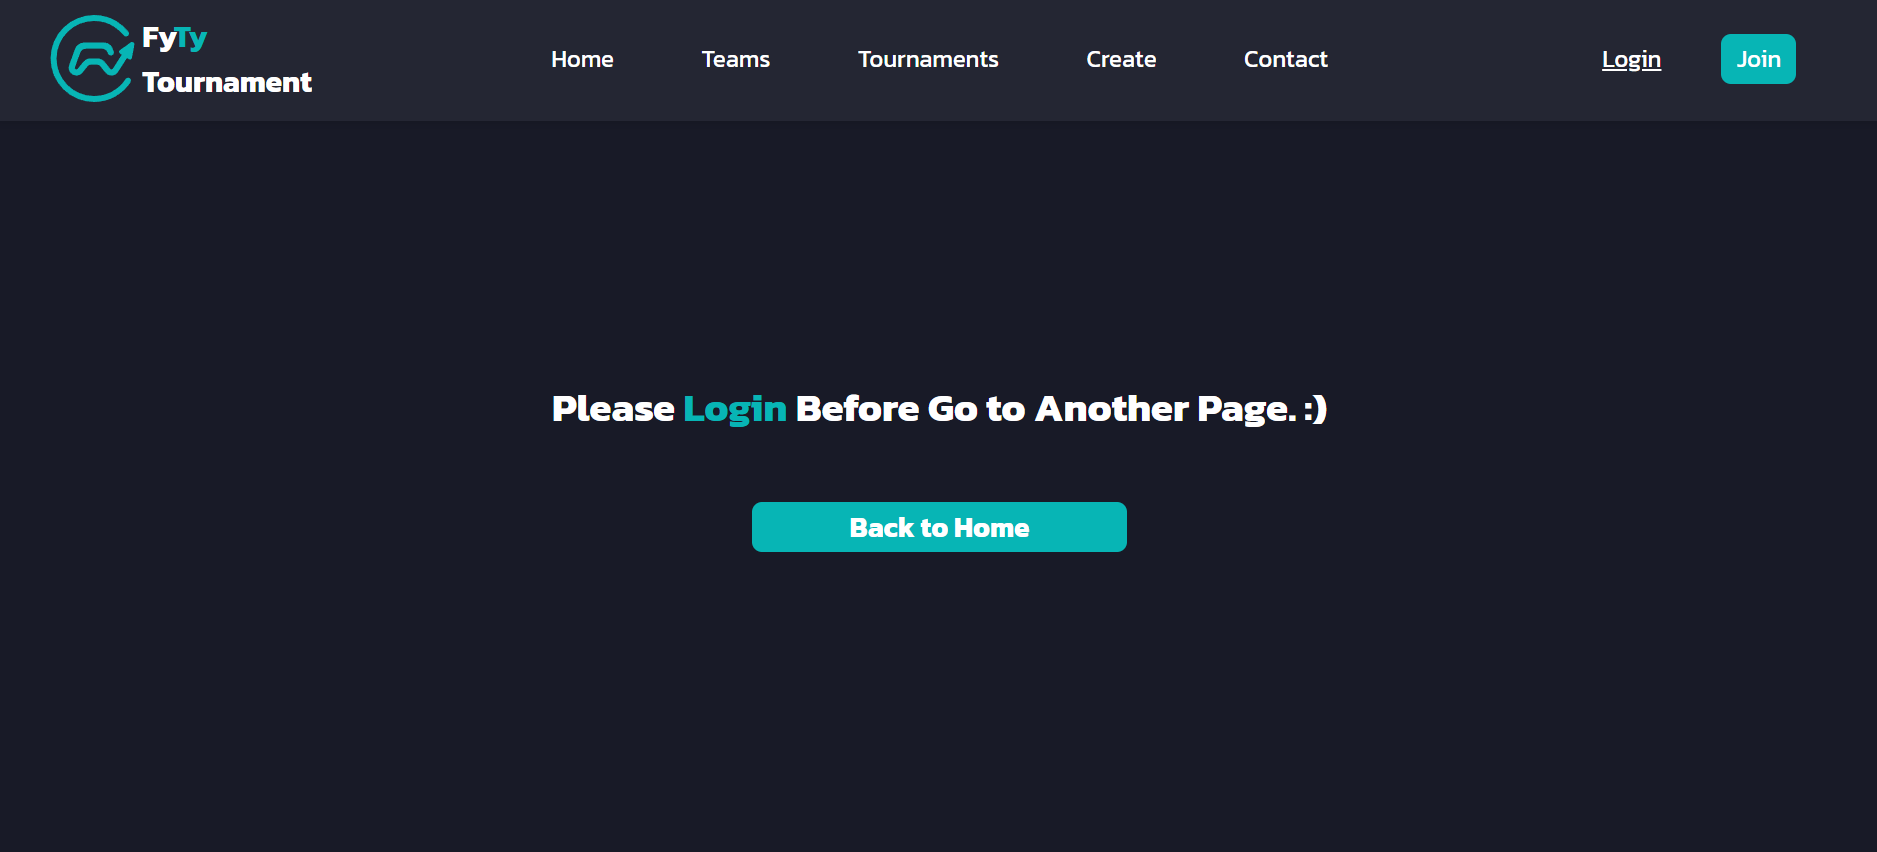
\includegraphics[width=18cm,height=7cm,keepaspectratio]{un_auth.png}
      \end{center}
      \caption[หน้าแจ้งเตือนหากไม่ได้ Login]{หน้าแจ้งเตือนหากไม่ได้ Login}
      \label{fig:หน้าแจ้งเตือนหากไม่ได้ Login}
    \end{figure}

    % team
    \begin{figure}[ht]
      \begin{center}
      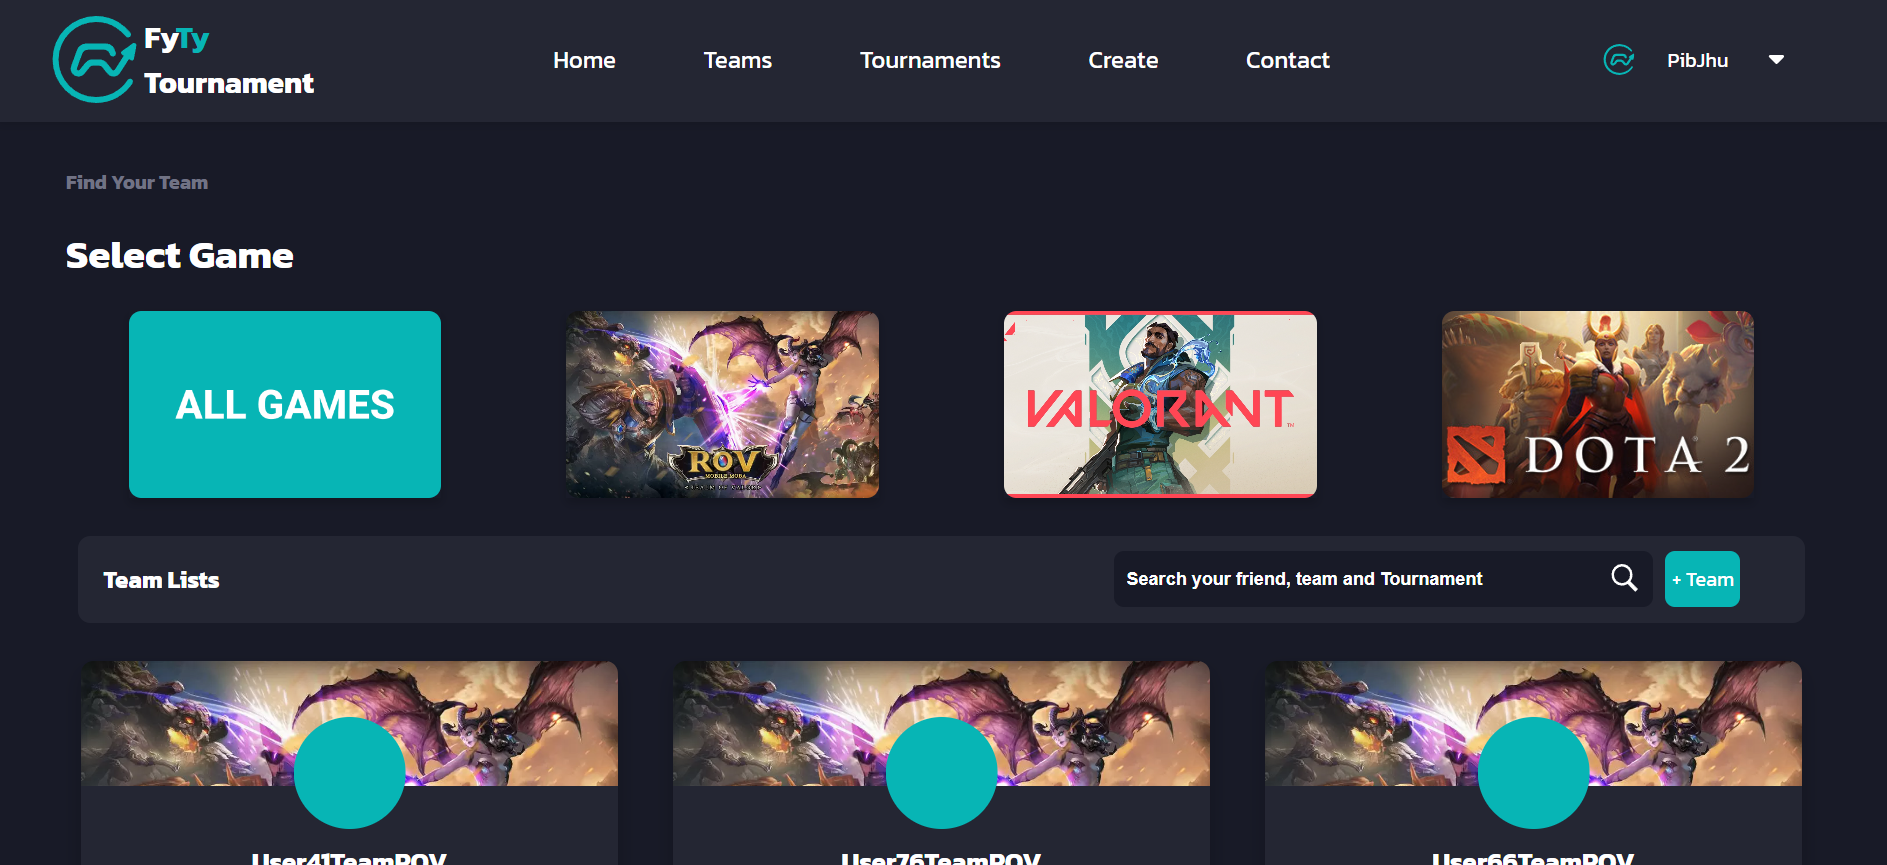
\includegraphics[width=18cm,height=7cm,keepaspectratio]{team.png}
      \end{center}
      \caption[หน้าเดชบอร์ดทีม]{หน้าเดชบอร์ดทีม}
      \label{fig:หน้าเดชบอร์ดทีม}
    \end{figure}
    \begin{figure}[ht]
      \begin{center}
      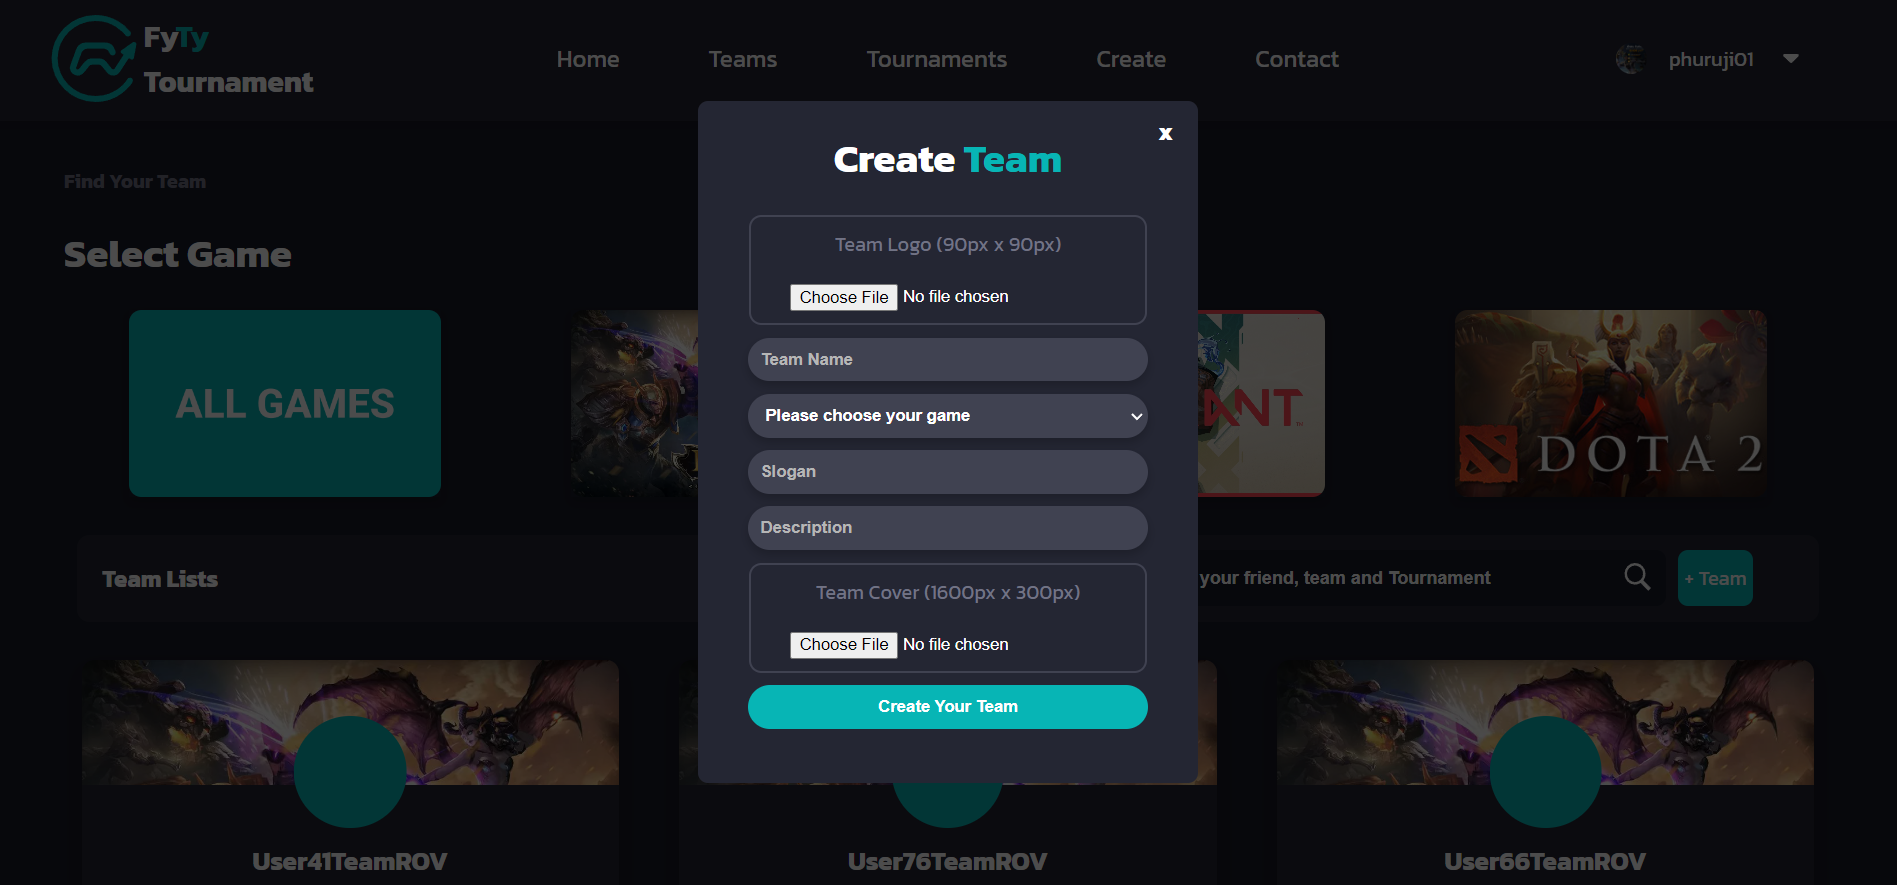
\includegraphics[width=18cm,height=7cm,keepaspectratio]{team_create.png}
      \end{center}
      \caption[Create Team Popup]{Create Team Popup}
      \label{fig:Create Team Popup}
    \end{figure}

    % team each
    \begin{figure}[ht]
      \begin{center}
      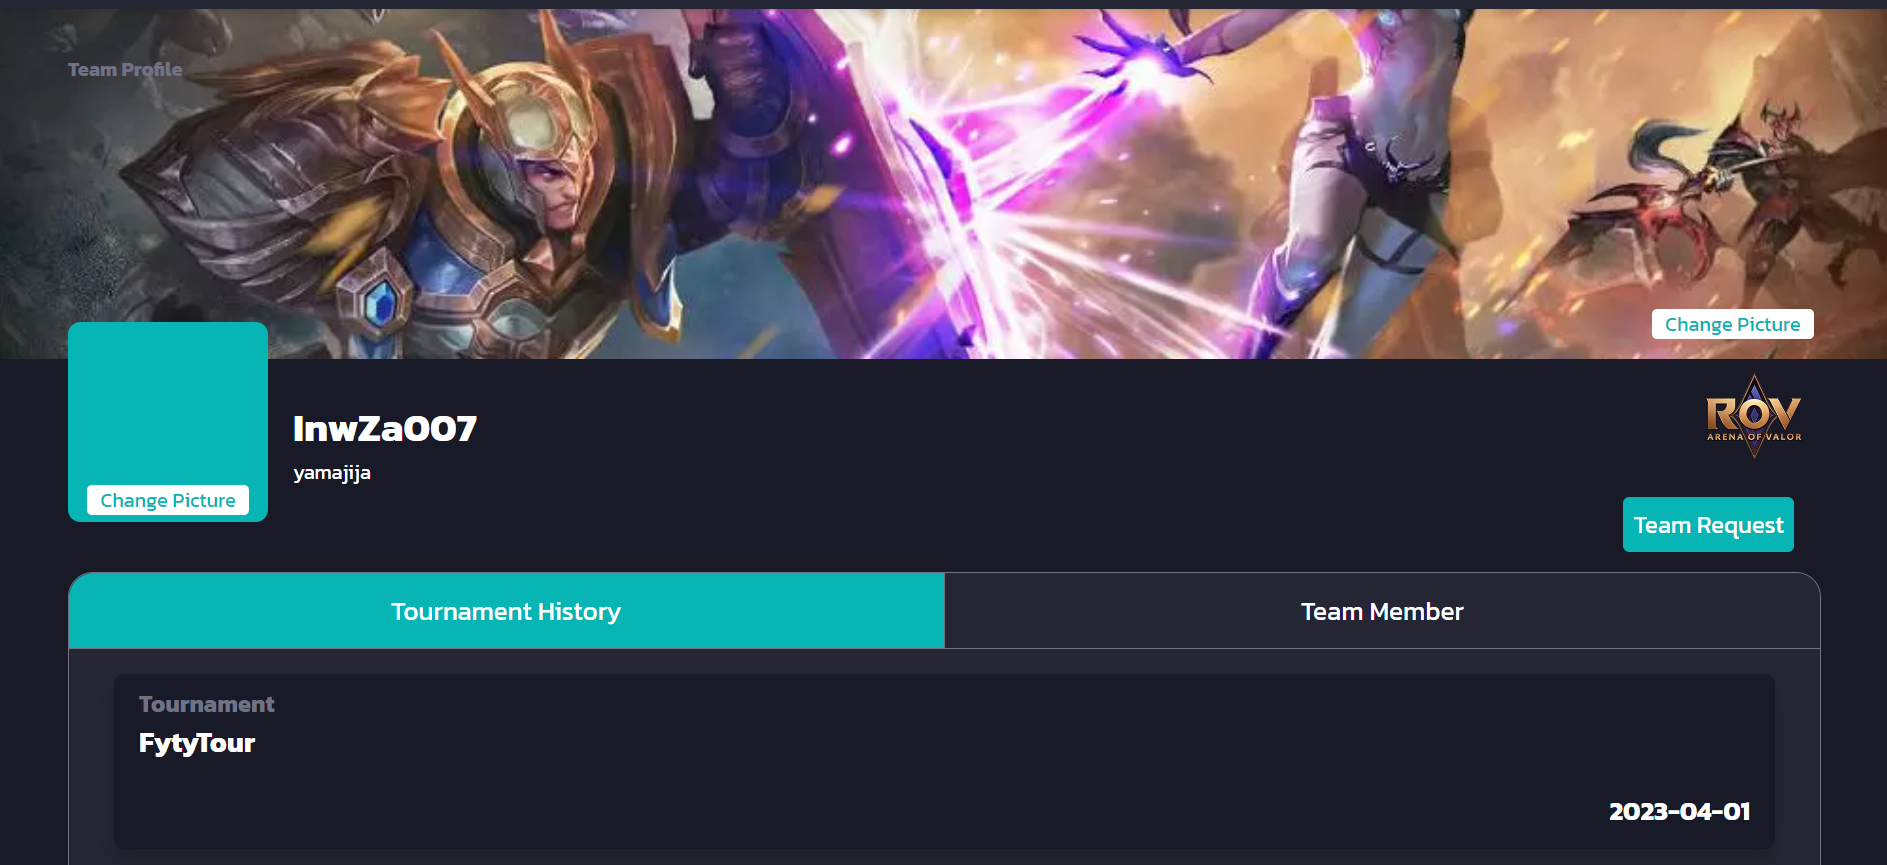
\includegraphics[width=18cm,height=7cm,keepaspectratio]{team_each_th.png}
      \end{center}
      \caption[หน้ารายละเอียดทีม และประวัติการแข่งขัน]{หน้ารายละเอียดทีม และประวัติการแข่งขัน}
      \label{fig:หน้ารายละเอียดทีม และประวัติการแข่งขัน}
    \end{figure}
    \begin{figure}[ht]
      \begin{center}
      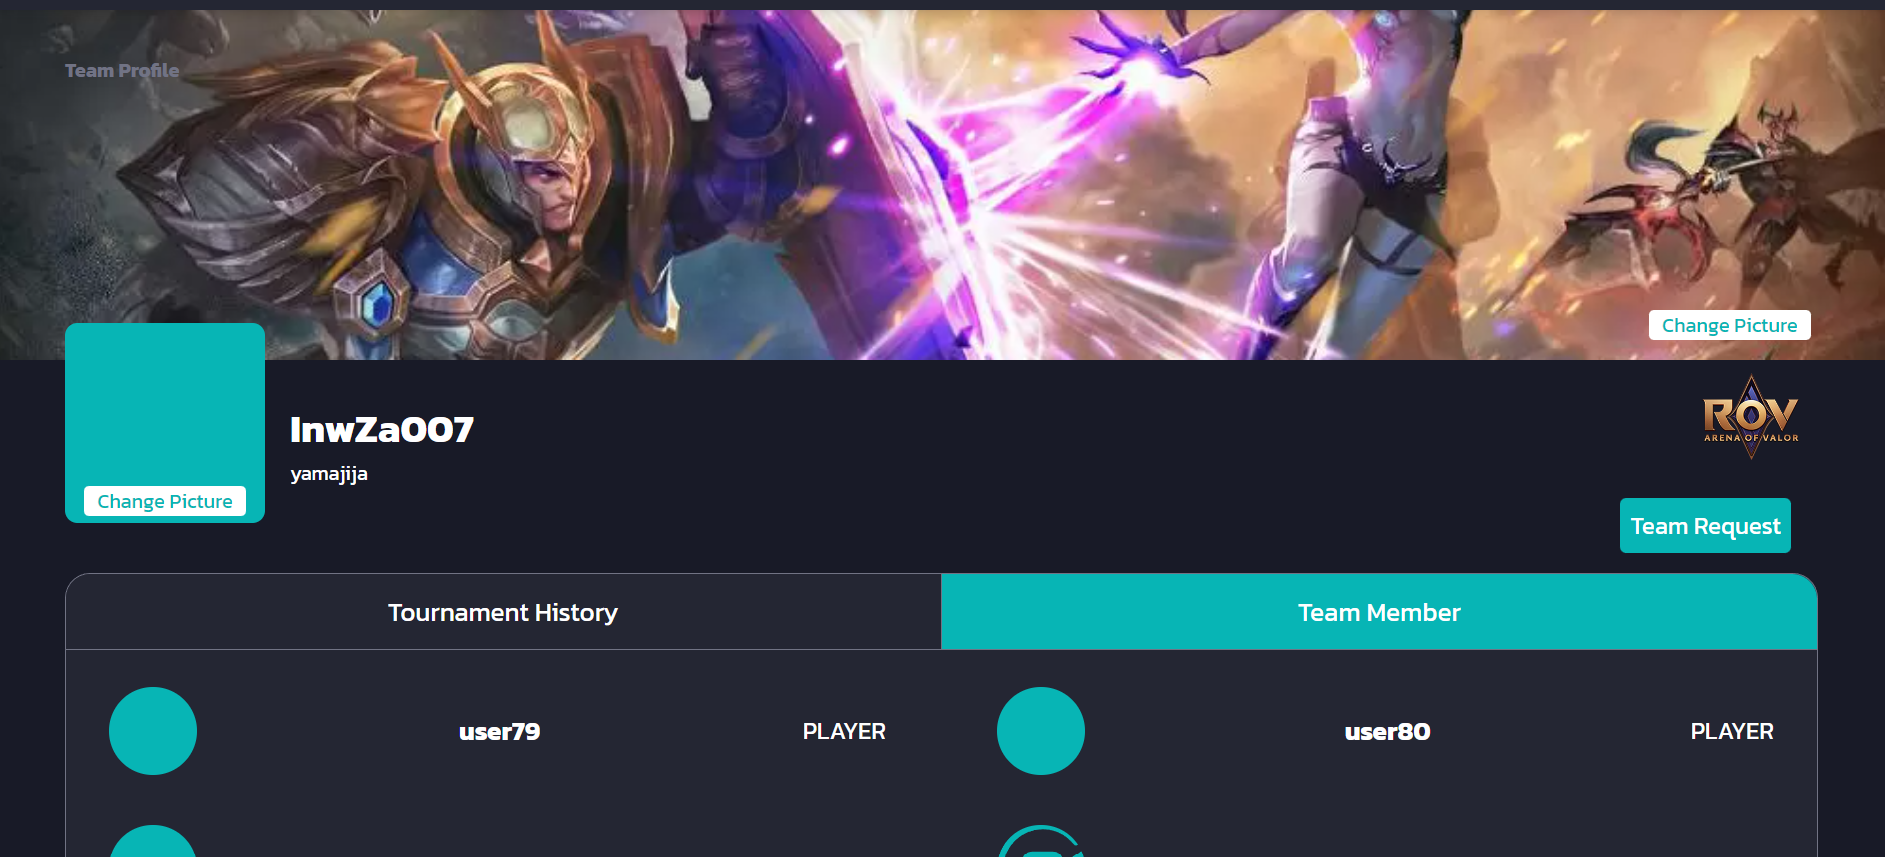
\includegraphics[width=18cm,height=7cm,keepaspectratio]{team_each_tm.png}
      \end{center}
      \caption[หน้ารายละเอียดทีม และสมาชิกทีม]{หน้ารายละเอียดทีม และสมาชิกทีม}
      \label{fig:หน้ารายละเอียดทีม และสมาชิกทีม}
    \end{figure}
    \begin{figure}[ht]
      \begin{center}
      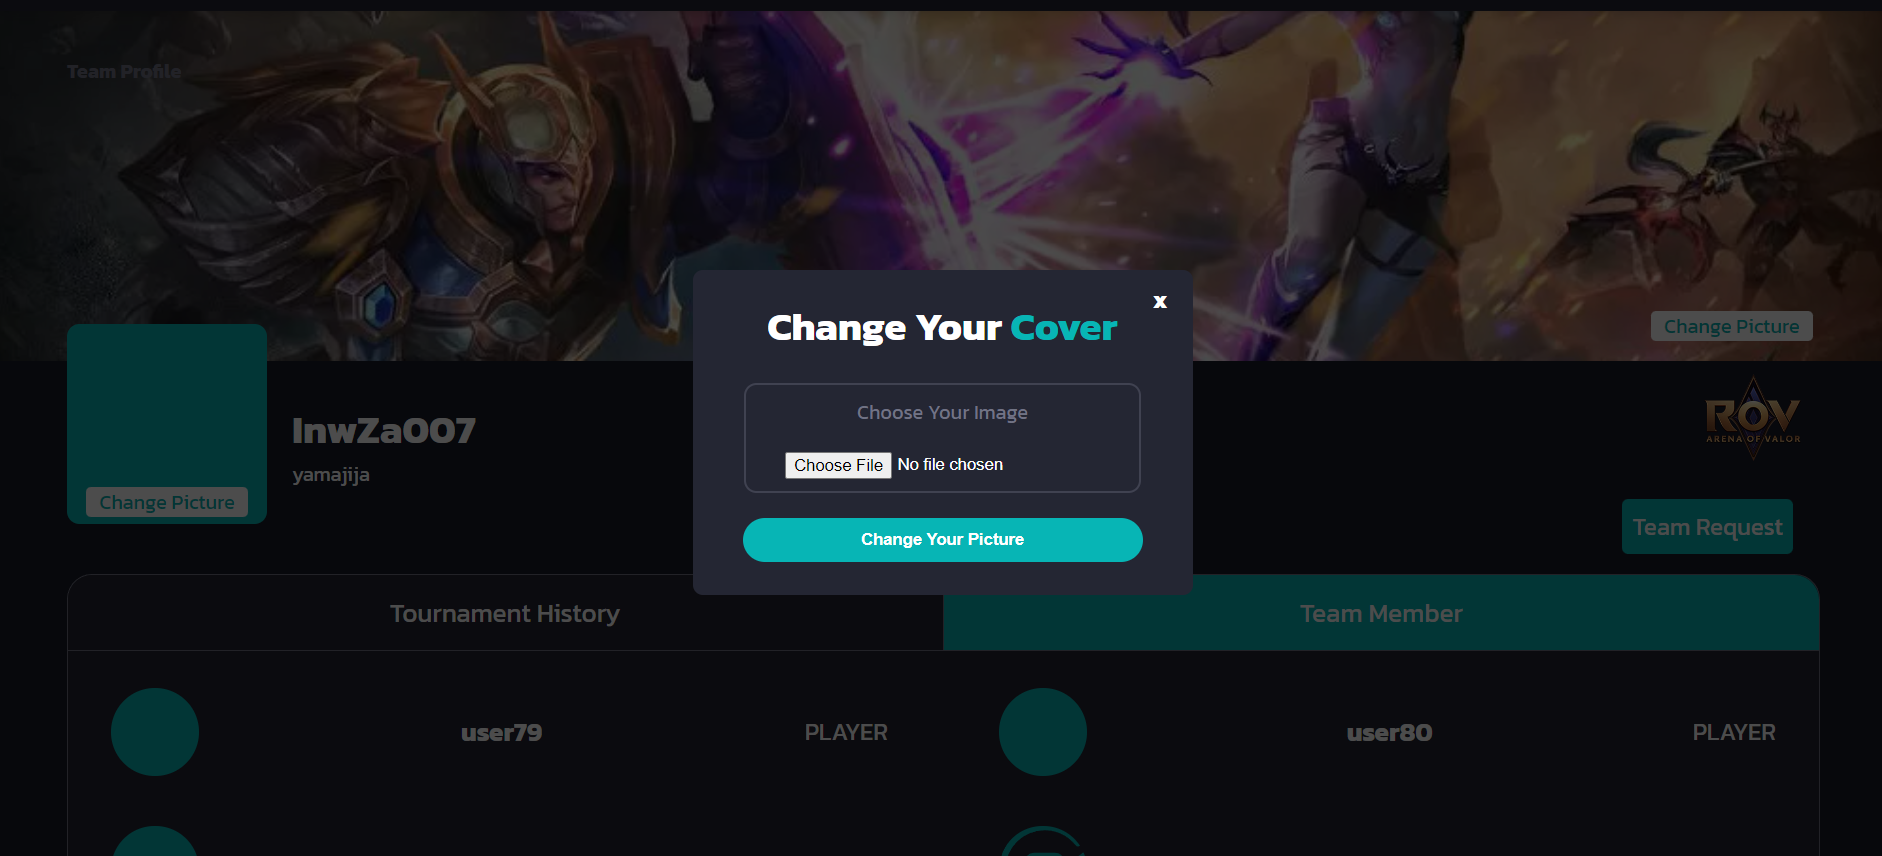
\includegraphics[width=18cm,height=7cm,keepaspectratio]{team_each_change_pic.png}
      \end{center}
      \caption[Create Picture Popup]{Create Picture Popup}
      \label{fig:Change Picture Popup}
    \end{figure}

    % tournmanet
    \begin{figure}[ht]
      \begin{center}
      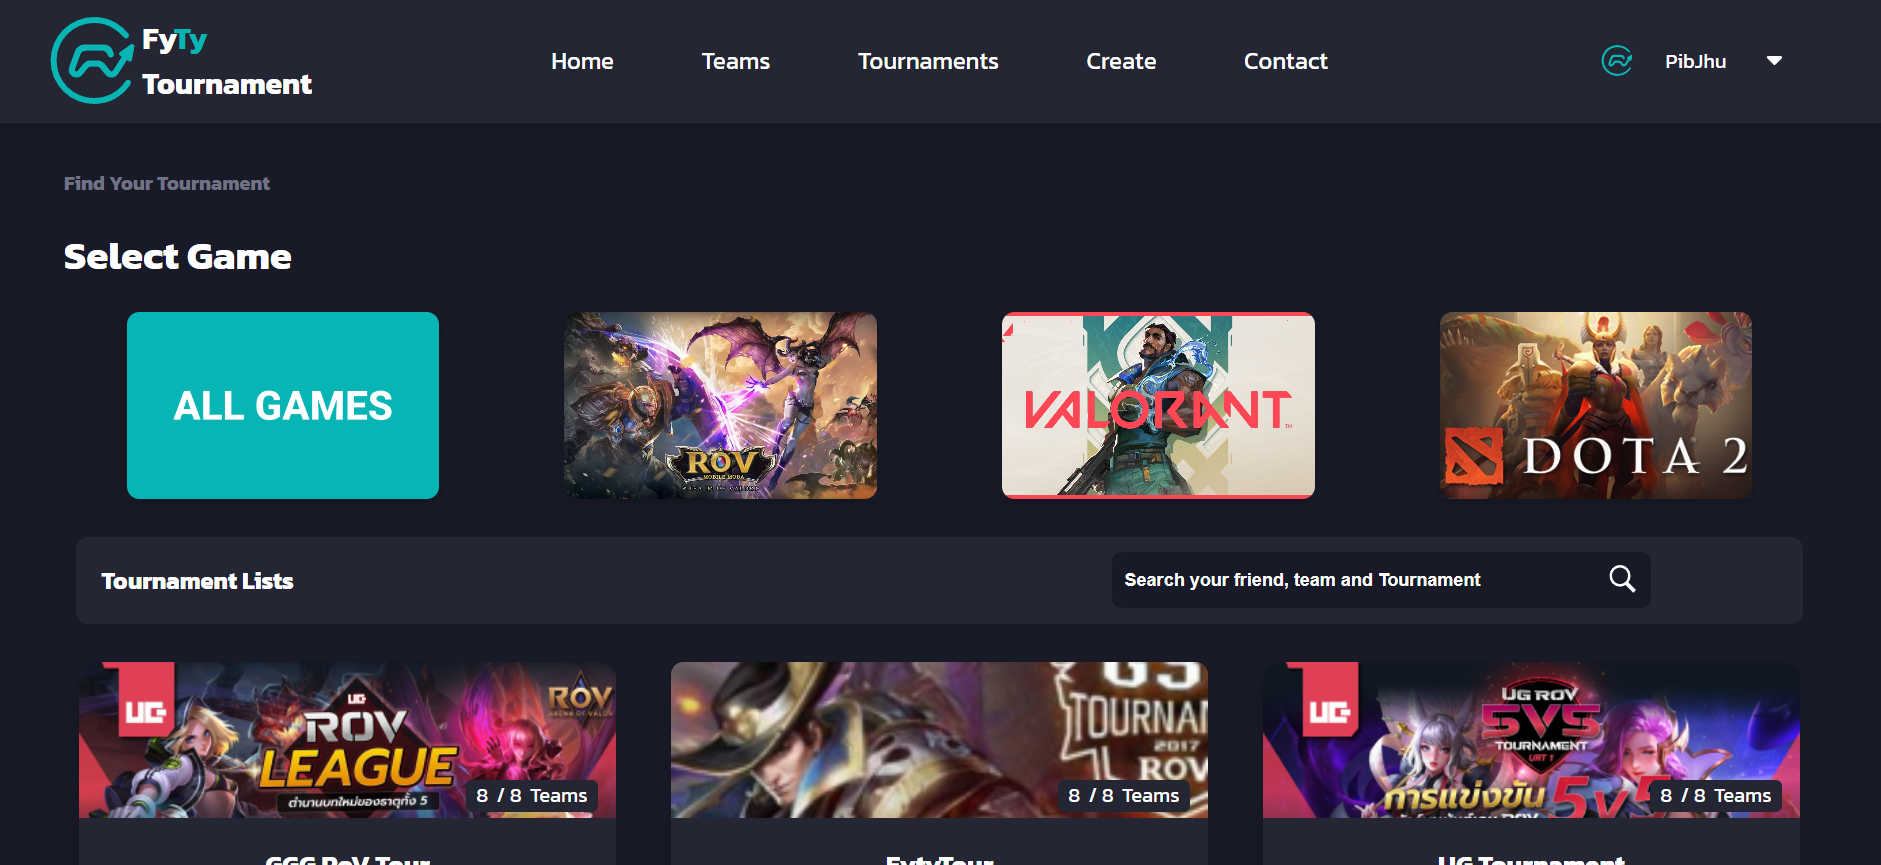
\includegraphics[width=18cm,height=7cm,keepaspectratio]{tournament.png}
      \end{center}
      \caption[หน้าแดชบอร์ดทัวร์นาเมนต์]{หน้าแดชบอร์ดทัวร์นาเมนต์}
      \label{fig:หน้าแดชบอร์ดทัวร์นาเมนต์}
    \end{figure}
    % tournament each
    \begin{figure}[ht]
      \begin{center}
      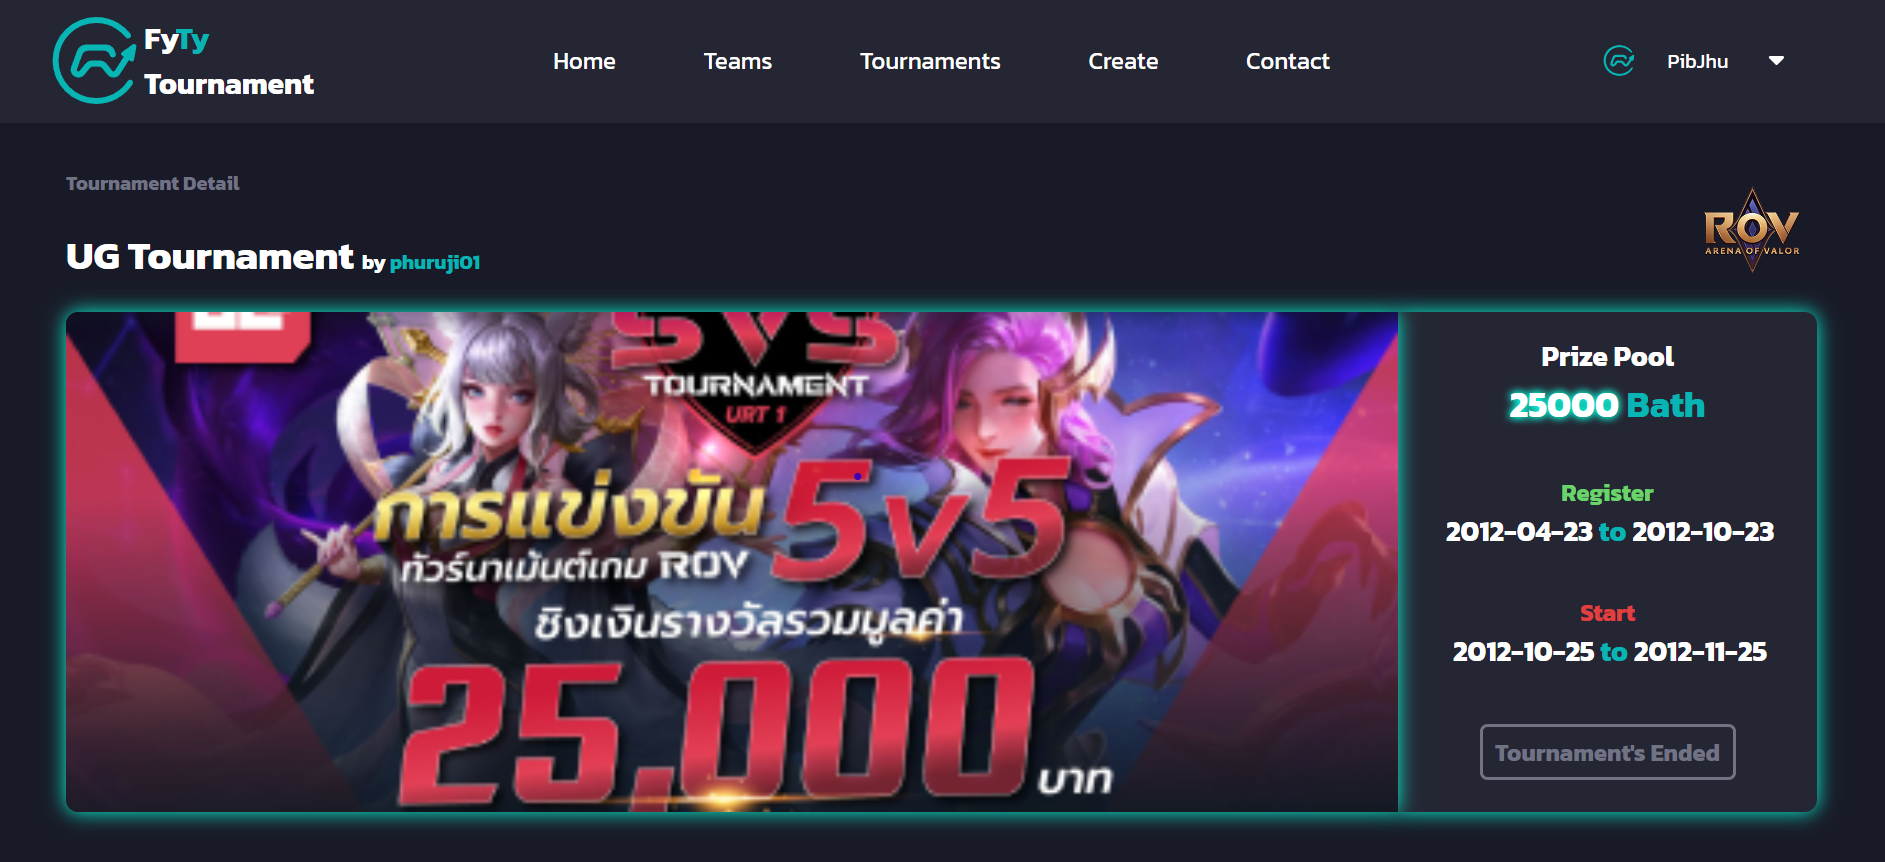
\includegraphics[width=18cm,height=7cm,keepaspectratio]{tournament_each_detail.png}
      \end{center}
      \caption[หน้ารายละเอียดทัวร์นาเมนต์(รายละเอียดทัวร์นาเมนต์)]{หน้ารายละเอียดทัวร์นาเมนต์(รายละเอียดทัวร์นาเมนต์)}
      \label{fig:หน้ารายละเอียดทัวร์นาเมนต์(รายละเอียดทัวร์นาเมนต์)}
    \end{figure}
    \begin{figure}[ht]
      \begin{center}
      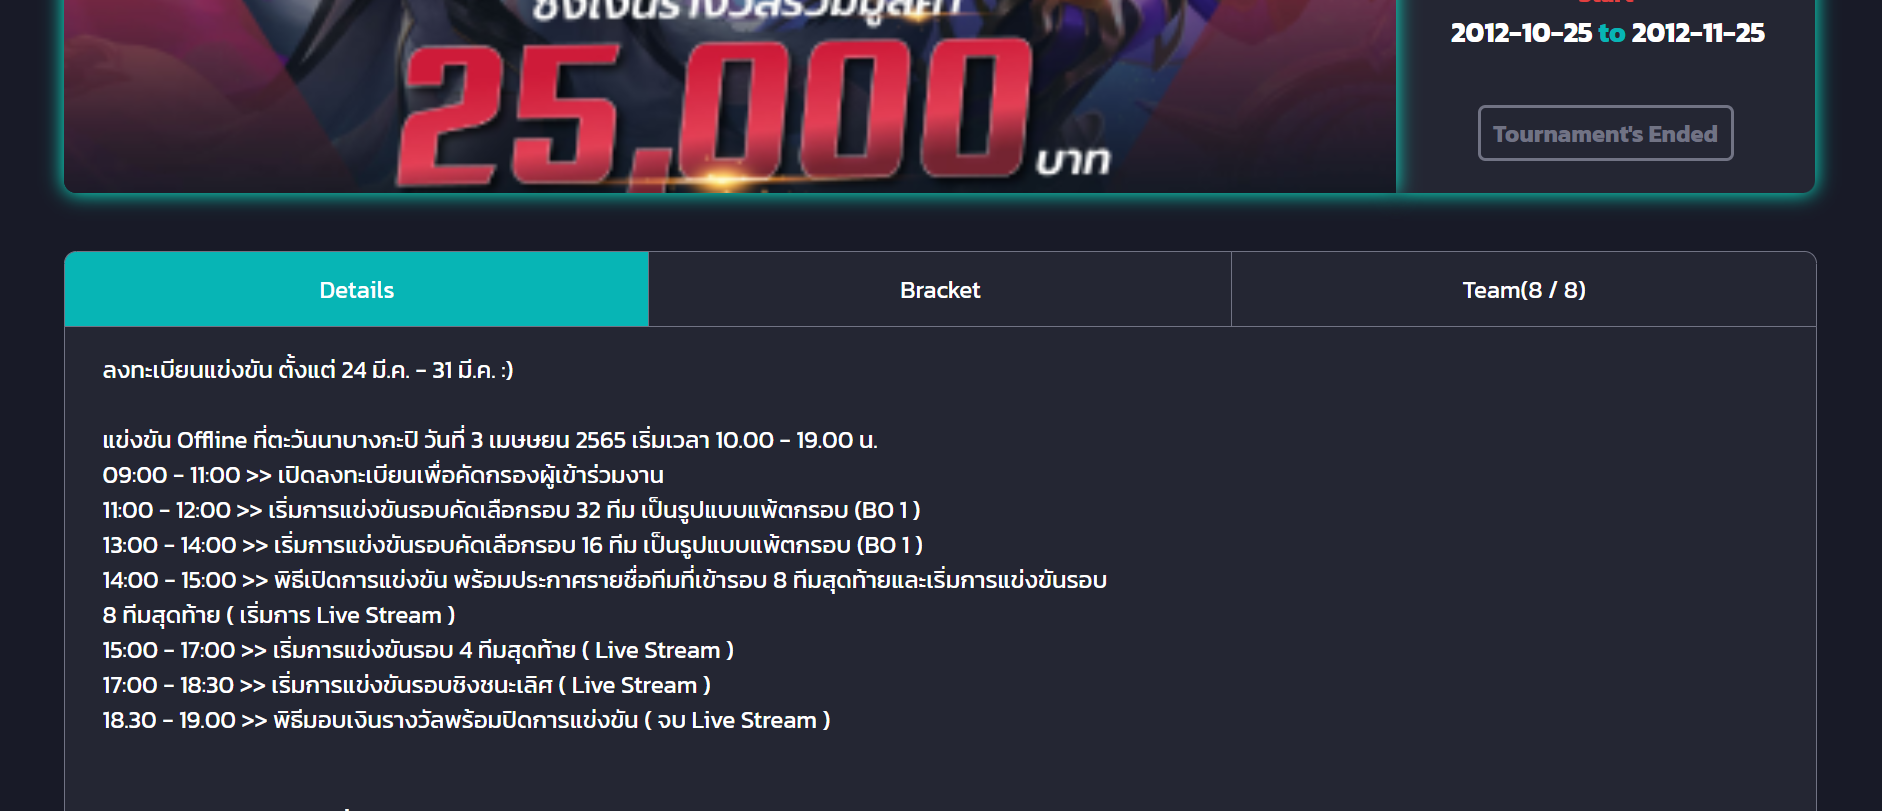
\includegraphics[width=18cm,height=7cm,keepaspectratio]{tournament_each_rule.png}
      \end{center}
      \caption[หน้ารายละเอียดทัวร์นาเมนต์(รายละเอียดการแข่ง)]{หน้ารายละเอียดทัวร์นาเมนต์(รายละเอียดการแข่ง)}
      \label{fig:หน้ารายละเอียดทัวร์นาเมนต์(รายละเอียดการแข่ง)}
    \end{figure}
    \begin{figure}[ht]
      \begin{center}
      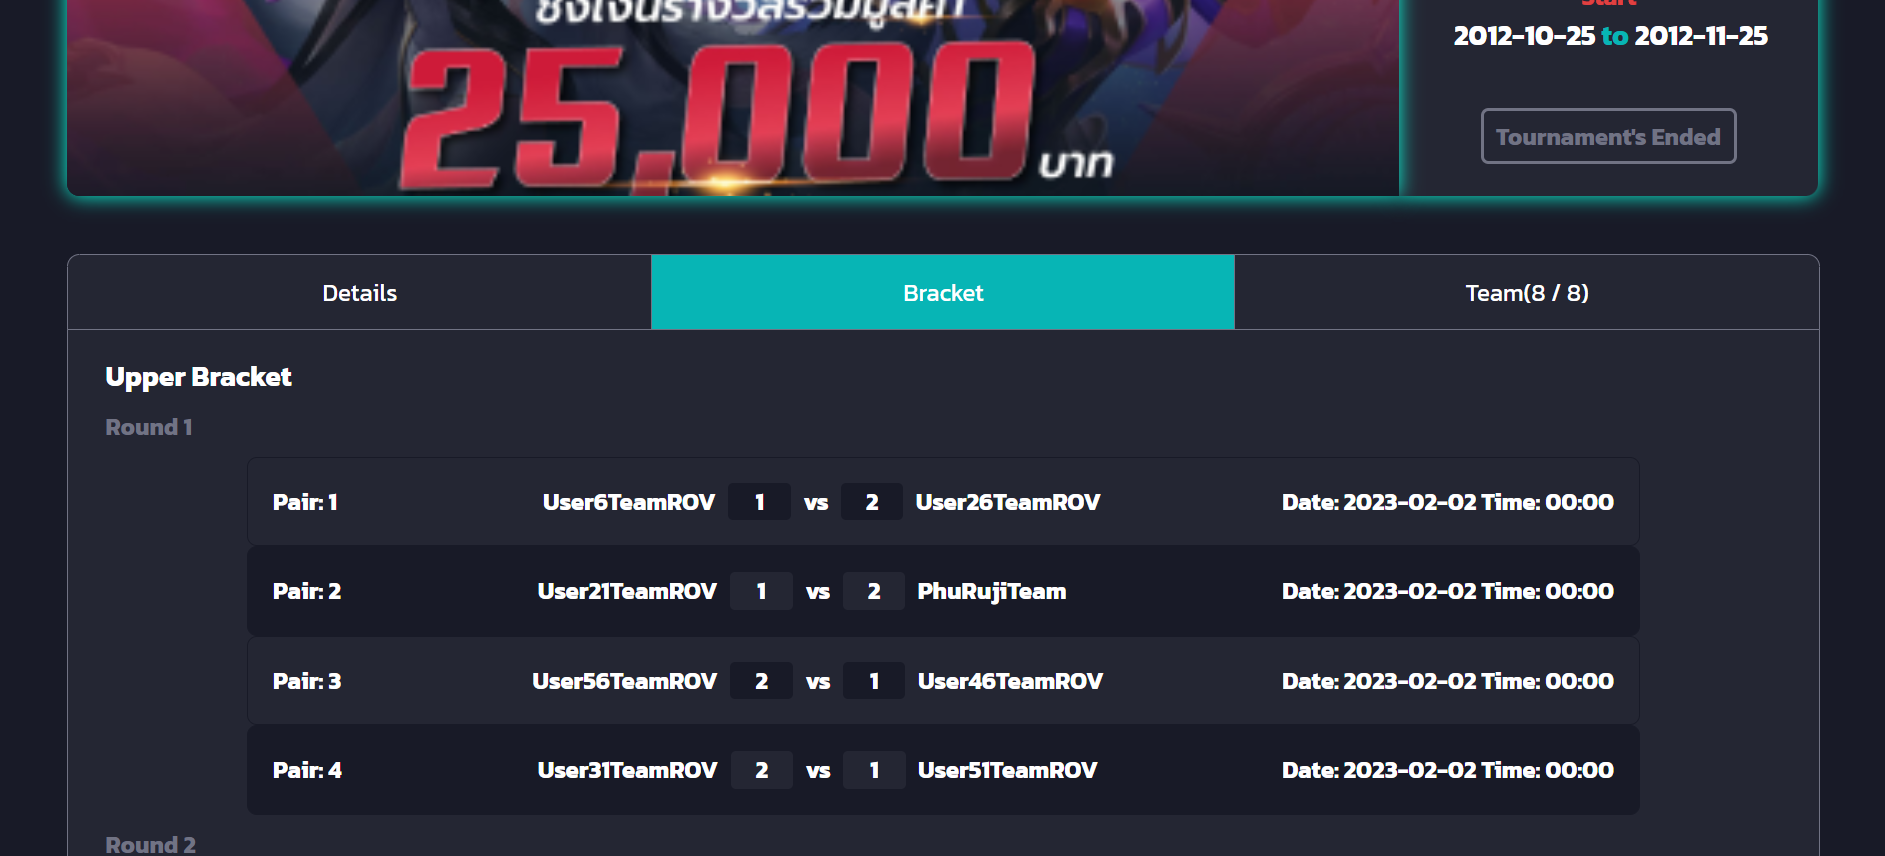
\includegraphics[width=18cm,height=7cm,keepaspectratio]{tournament_each_bracket.png}
      \end{center}
      \caption[หน้ารายละเอียดทัวร์นาเมนต์(ตารางเเข่ง)]{หน้ารายละเอียดทัวร์นาเมนต์(ตารางเเข่ง)}
      \label{fig:หน้ารายละเอียดทัวร์นาเมนต์(ตารางเเข่ง)}
    \end{figure}
    \begin{figure}[ht]
      \begin{center}
      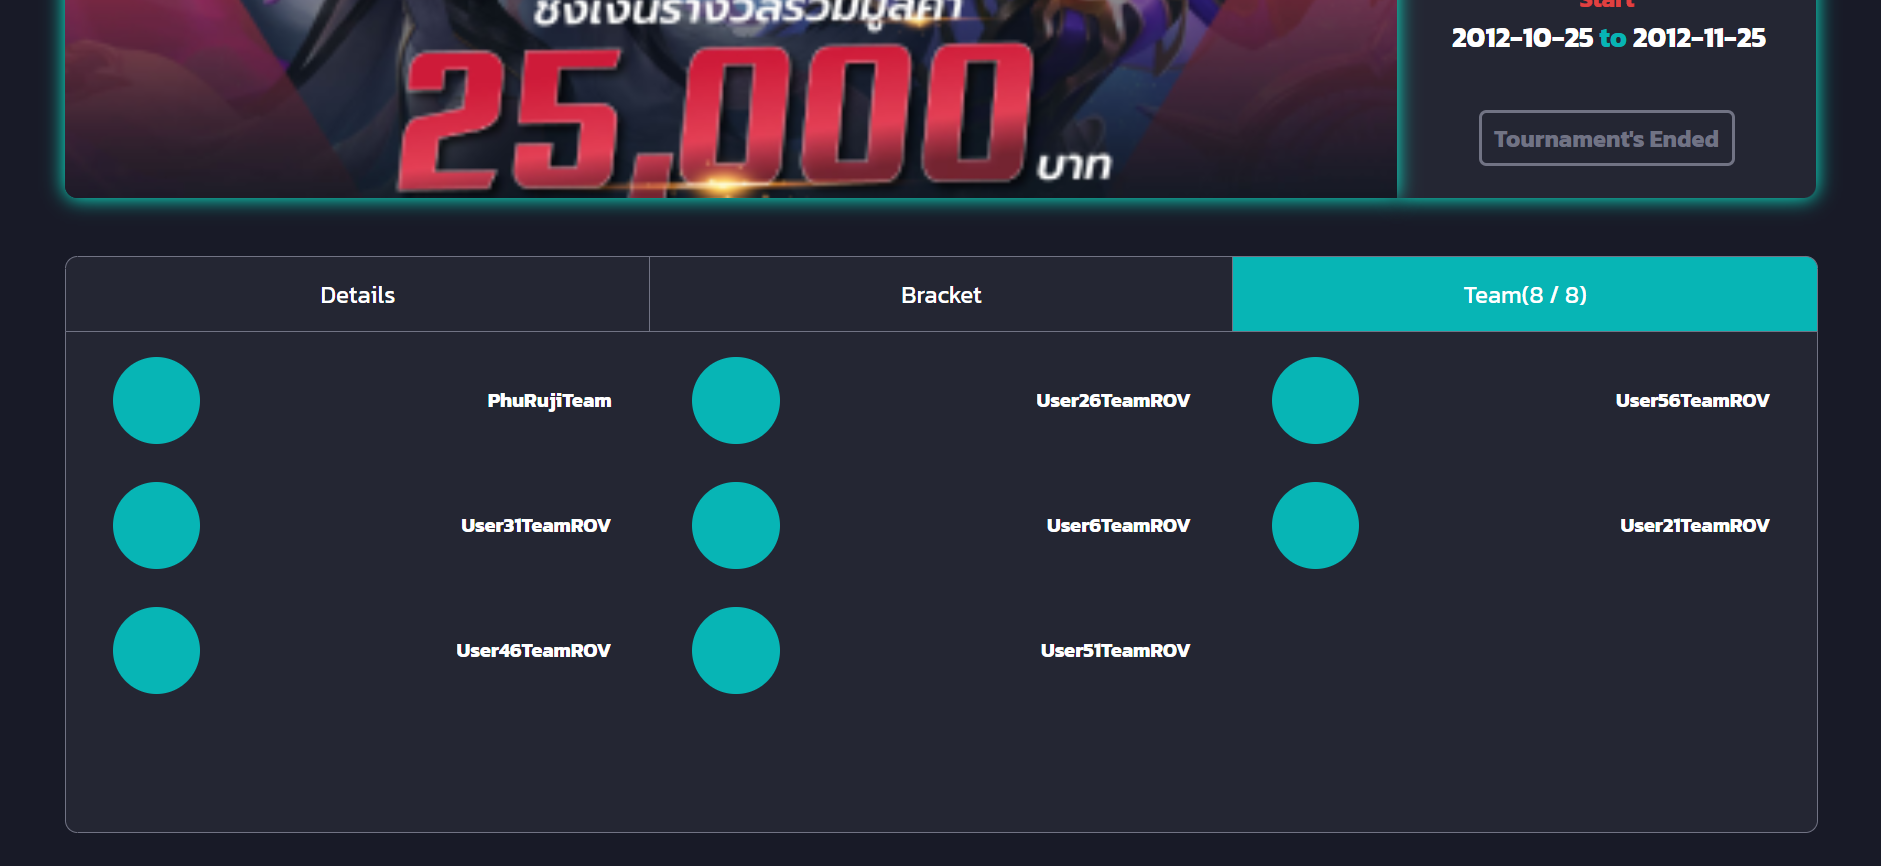
\includegraphics[width=18cm,height=7cm,keepaspectratio]{tournament_each_tj.png}
      \end{center}
      \caption[หน้ารายละเอียดทัวร์นาเมนต์(ทีมที่เข้าร่วม)]{หน้ารายละเอียดทัวร์นาเมนต์(ทีมที่เข้าร่วม)}
      \label{fig:หน้ารายละเอียดทัวร์นาเมนต์(ทีมที่เข้าร่วม)}
    \end{figure}
 
    % create
    \begin{figure}[ht]
      \begin{center}
      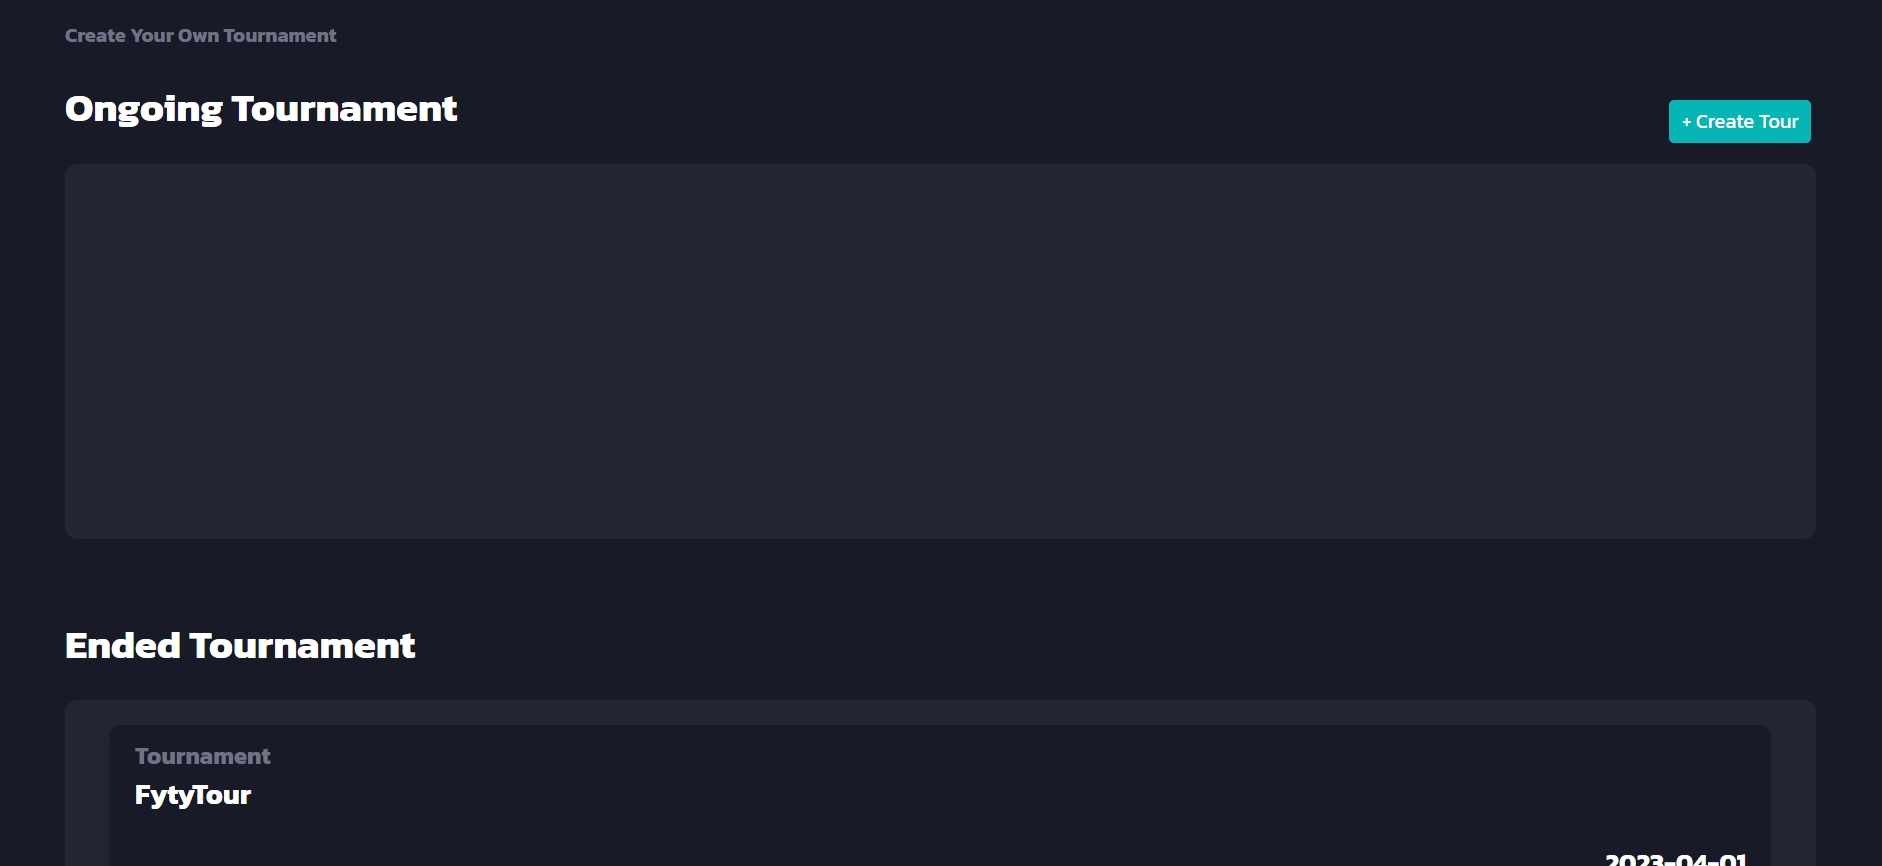
\includegraphics[width=18cm,height=7cm,keepaspectratio]{create_tour.png}
      \end{center}
      \caption[หน้าสร้างทัวร์นาเมนต์]{หน้าสร้างทัวร์นาเมนต์}
      \label{fig:หน้าสร้างทัวร์นาเมนต์}
    \end{figure}
    \begin{figure}[ht]
      \begin{center}
      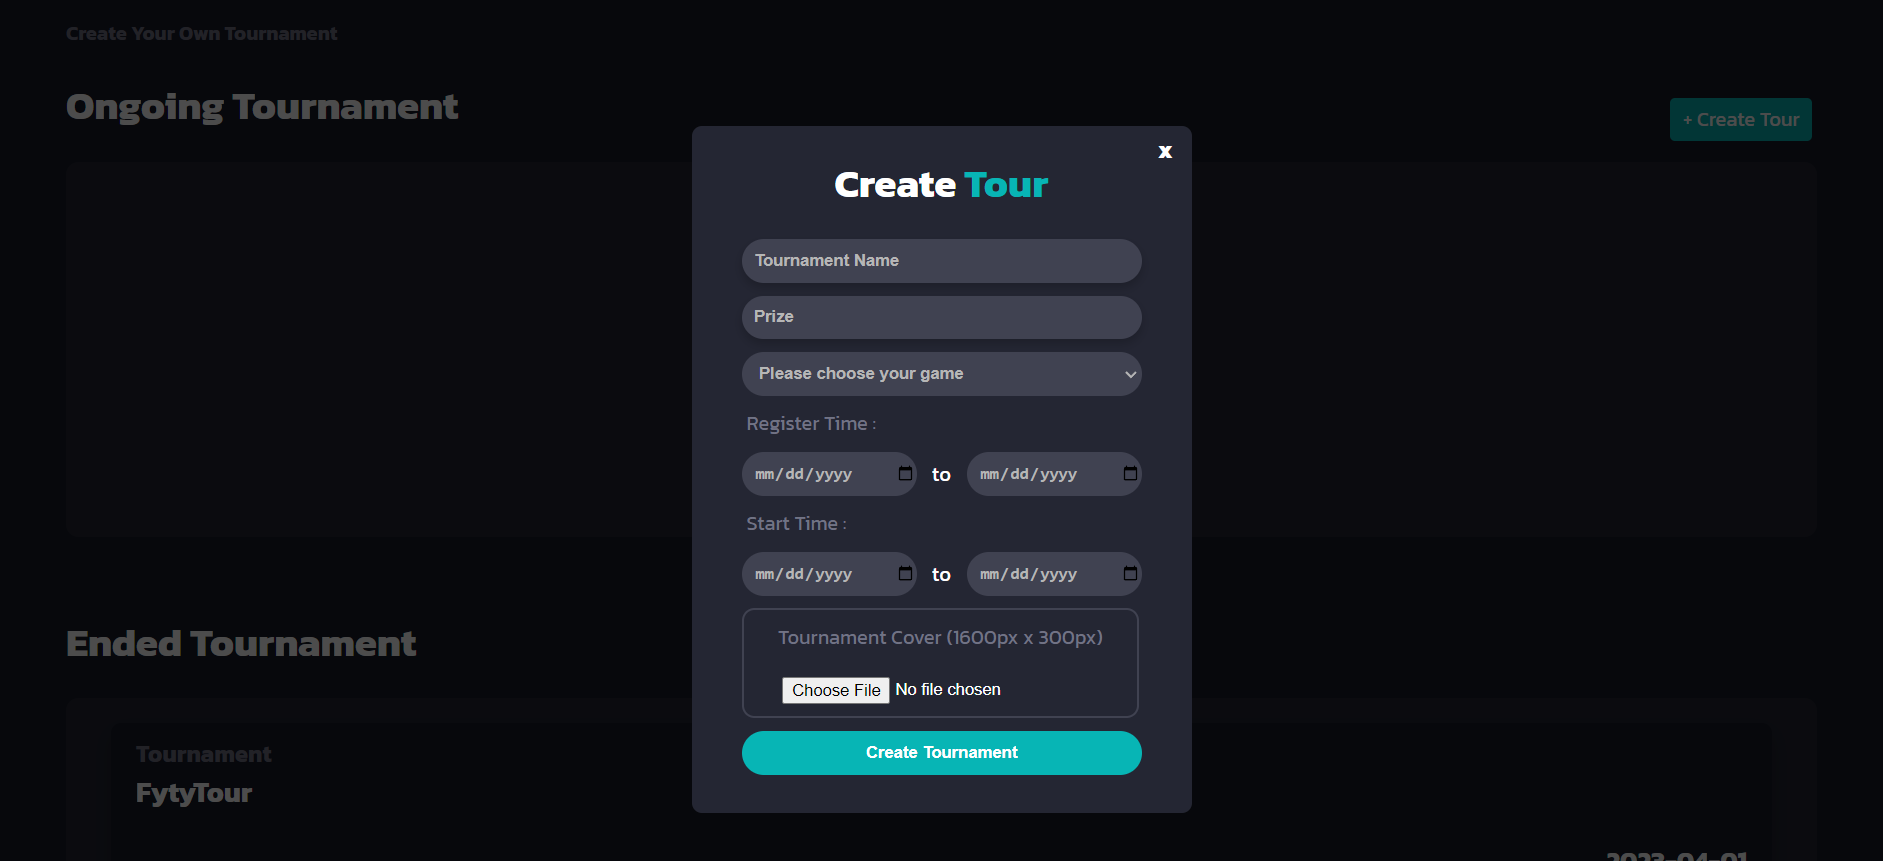
\includegraphics[width=18cm,height=7cm,keepaspectratio]{create_tour_popup.png}
      \end{center}
      \caption[Create Tournament Popup]{Create Tournament Popup}
      \label{fig:Create Tournament Popup}
    \end{figure}

    % profile
    \begin{figure}[ht]
      \begin{center}
      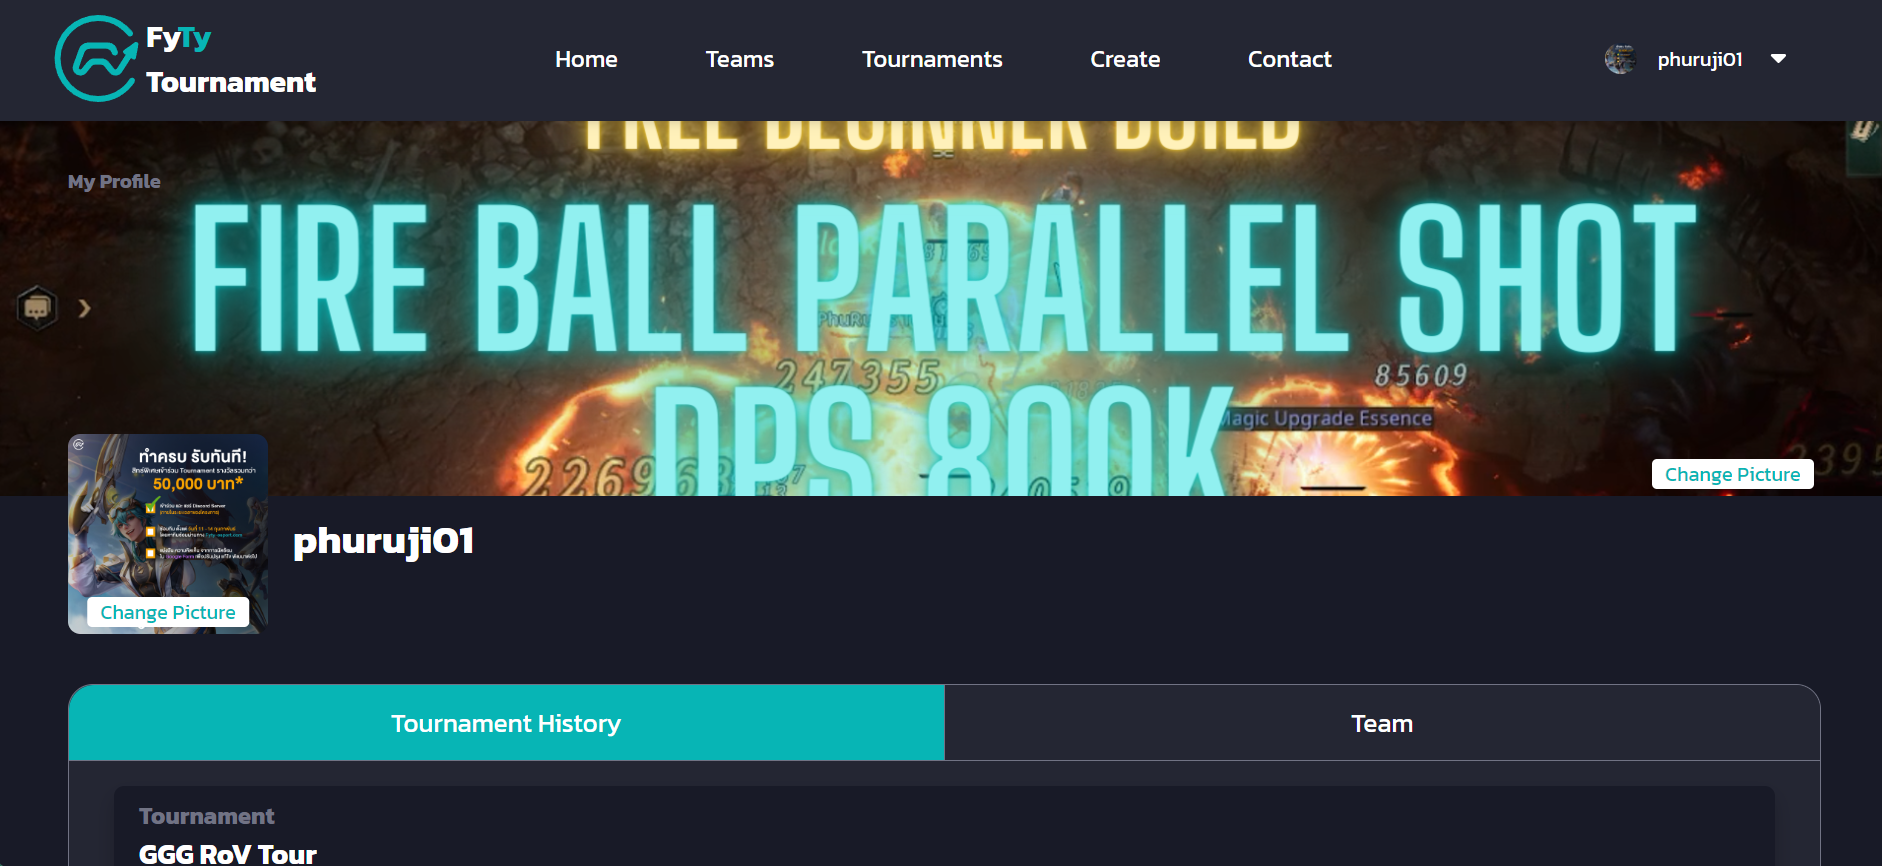
\includegraphics[width=18cm,height=7cm,keepaspectratio]{user_th.png}
      \end{center}
      \caption[หน้ารายละเอียดผู้ใช้(ประวัติการแข่ง)]{หน้ารายละเอียดผู้ใช้(ประวัติการแข่ง)}
      \label{fig:หน้ารายละเอียดผู้ใช้(ประวัติการแข่ง)}
    \end{figure}
    \begin{figure}[ht]
      \begin{center}
      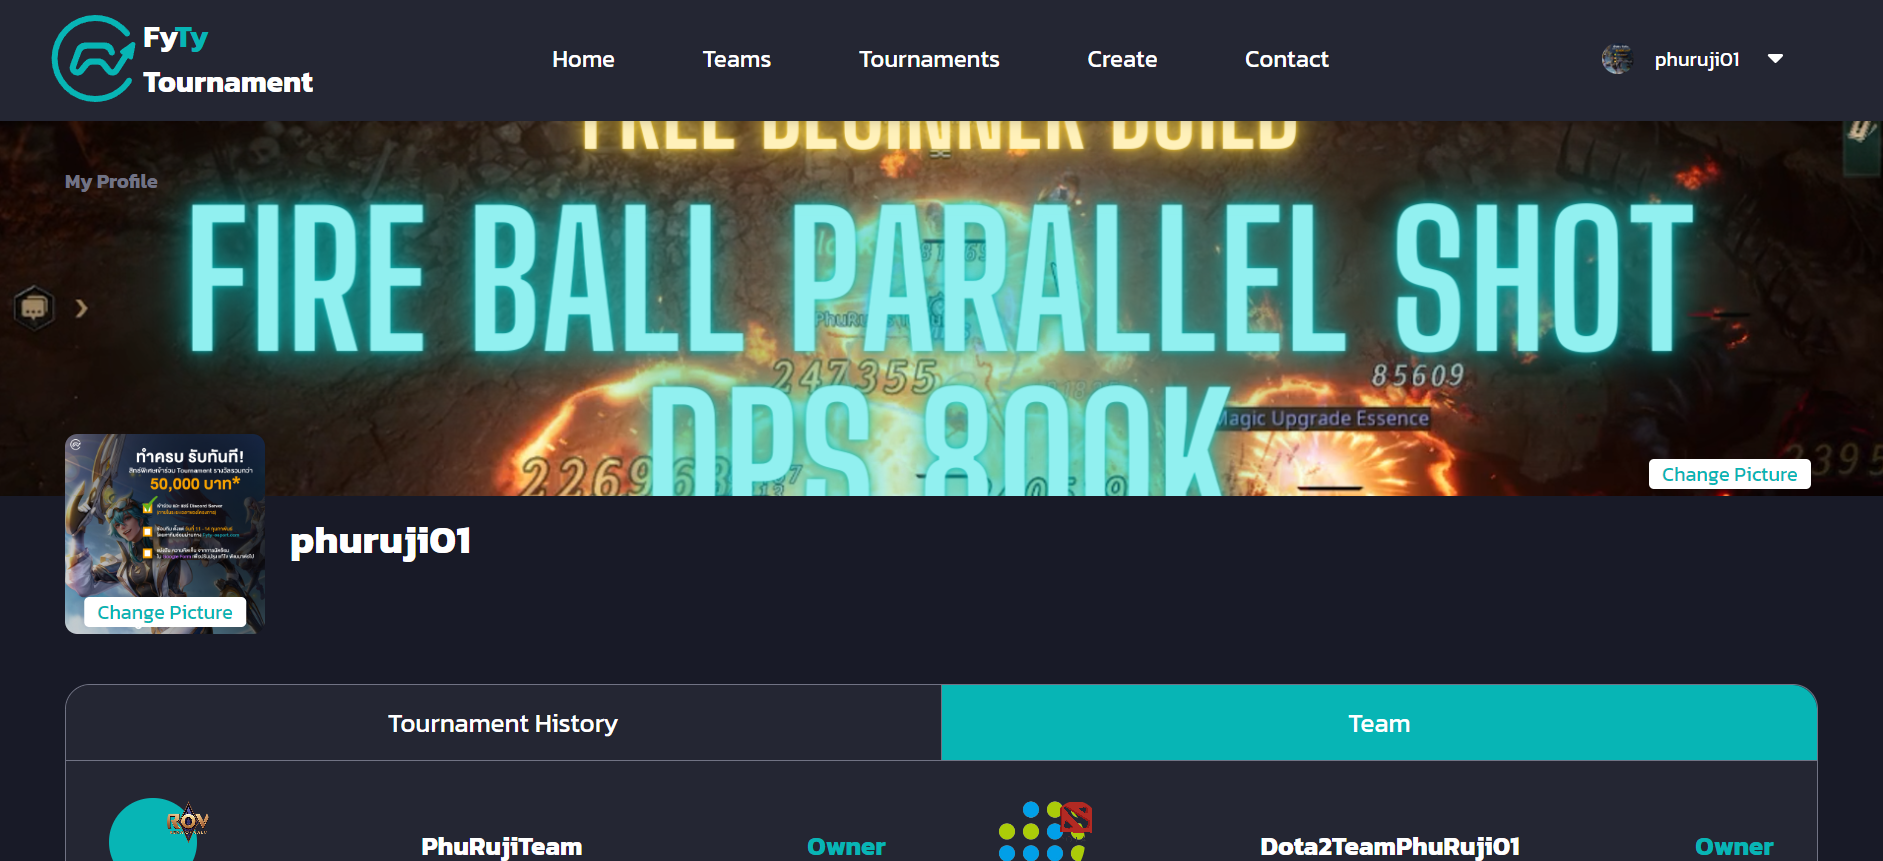
\includegraphics[width=18cm,height=7cm,keepaspectratio]{user_tj.png}
      \end{center}
      \caption[หน้ารายละเอียดผู้ใช้(ทีมที่เคยเข้าร่วม)]{หน้ารายละเอียดผู้ใช้(ทีมที่เคยเข้าร่วม)}
      \label{fig:หน้ารายละเอียดผู้ใช้(ทีมที่เคยเข้าร่วม)}
    \end{figure}

    % schedule
    \begin{figure}[ht]
      \begin{center}
      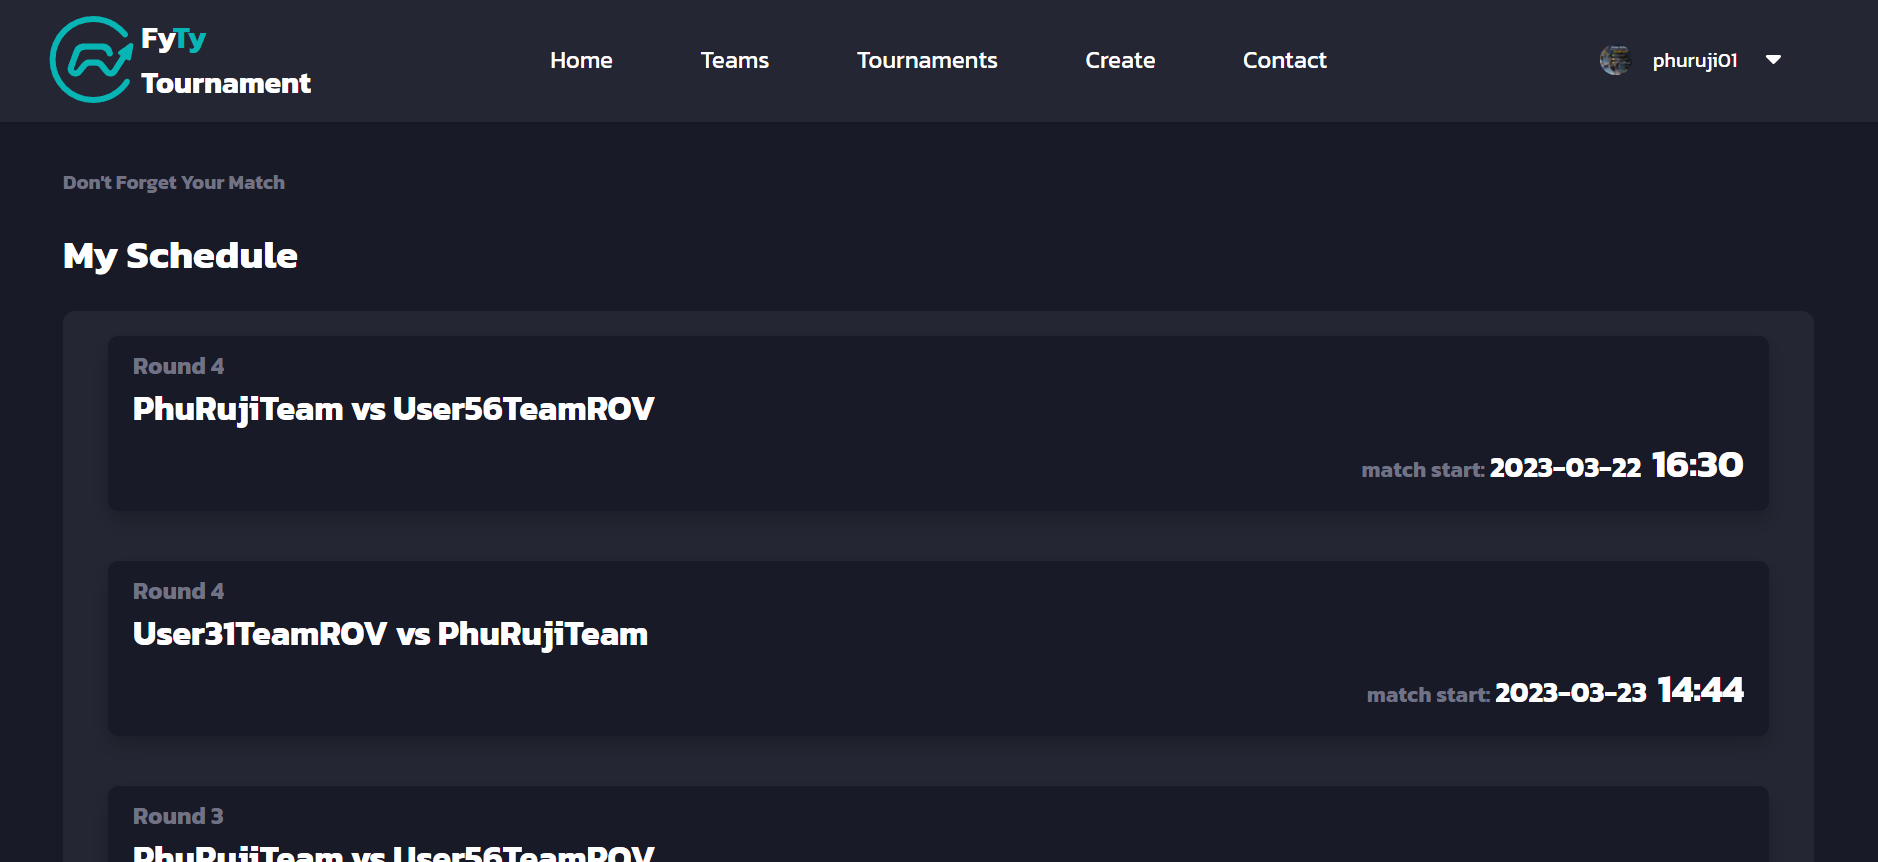
\includegraphics[width=18cm,height=7cm,keepaspectratio]{schedule.png}
      \end{center}
      \caption[ตารางแข่งของเรา]{ตารางแข่งของเรา}
      \label{fig:ตารางแข่งของเรา}
    \end{figure}



